
\subsection{Polarización}

\par Se simularon los valores en reposo de los transistores de la etapa amplificadora clase G, junto con la máxima potencia disipada en cada uno. Los resultados se muestran en el cuadro ~\tableref{table:PuntoQ_simulacion}\\

\begin{table}[H]  %%\centering
    
    \setlength\arrayrulewidth{1.5pt}
    \arrayrulecolor{white}
    \def\clinecolor{\hhline{|>{\arrayrulecolor{white}}-%
    >{\arrayrulecolor{white}}|-|-|-|-|-|}}
    
\begin{center}  
\resizebox{0.7 \textwidth}{!}{%    
\begin{tabularx}{1 \textwidth}%
    {|
    >{\columncolor{white} \centering\arraybackslash}m{0.3333\linewidth}
     |
    >{\columncolor{white} \centering\arraybackslash}m{0.1667\linewidth}
     |
    >{\columncolor{white} \centering\arraybackslash}m{0.1667\linewidth}
     |
    >{\columncolor{white} \centering\arraybackslash}m{0.1667\linewidth}
     |
    >{\columncolor{white} \centering\arraybackslash}m{0.1667\linewidth}
     |
    }
    \rowcolor{HeadersColor} \thead{Transistor} & \thead{$V_{BE_{Q}}$} & \thead{$V_{CE_{Q}}$} & \thead{$I_{C_{Q}}$} & \thead{ $P_{Q}$}\\    
    \hhline{|-|-|-|-|-|}
    %\rowcolor{Butter!20} \cellcolor{Butter!40} $I_{C}$ [$\si[per-mode=symbol]{\milli\ampere}$] & $0.54$ & $8.66$ & $9$ & $6$ & $5.5$ & $10$ & $10$  \\
    % \hhline{|-|-|-|-|-|}
    \rowcolor{gray!20} \cellcolor{gray!40} $Q_{1}$ (BC546C) & $612 \si[per-mode=symbol]{\milli\volt}$ & $33.87 \si[per-mode=symbol]{\volt}$ &  $549 \si[per-mode=symbol]{\micro\ampere}$ & $18.6 \si[per-mode=symbol]{\milli\watt}$ \\
    \hhline{|-|-|-|-|-|}
    \rowcolor{gray!20} \cellcolor{gray!40} $Q_{2}$ (BC556B) & $-610 \si[per-mode=symbol]{\milli\volt} $ & $-1.31\si[per-mode=symbol]{\volt}$  & $549 \si[per-mode=symbol]{\micro\ampere} $ & $722\si[per-mode=symbol]{\micro\watt}$ \\
    \hhline{|-|-|-|-|-|}
    \rowcolor{gray!20} \cellcolor{gray!40} $Q_{3}$ (BC546B) & $631\si[per-mode=symbol]{\milli\volt}$ & $31.78\si[per-mode=symbol]{\volt}$  & $1.1 \si[per-mode=symbol]{\milli\ampere} $ & $35\si[per-mode=symbol]{\milli\watt} $ \\
    \hhline{|-|-|-|-|-|}
    \rowcolor{gray!20} \cellcolor{gray!40} $Q_{4}$ (BC556B) & $-610\si[per-mode=symbol]{\milli\volt}$ & $33.78\si[per-mode=symbol]{\volt}$  & $549 \si[per-mode=symbol]{\micro\ampere} $ & $334\si[per-mode=symbol]{\milli\watt}$ \\
    \hhline{|-|-|-|-|-|}
    \rowcolor{gray!20} \cellcolor{gray!40} $Q_{5}$ (BC546B) & $612\si[per-mode=symbol]{\milli\volt}$ & $34.6\si[per-mode=symbol]{\volt}$  & $549 \si[per-mode=symbol]{\micro\ampere} $ & $19\si[per-mode=symbol]{\milli\watt} $ \\
    \hhline{|-|-|-|-|-|}
    \rowcolor{gray!20} \cellcolor{gray!40} $Q_{6}$ (BC546B) & $693\si[per-mode=symbol]{\milli\volt}$ & $28.8\si[per-mode=symbol]{\volt}$  & $9.71 \si[per-mode=symbol]{\milli\ampere} $ & $280\si[per-mode=symbol]{\milli\watt}$ \\
    \hhline{|-|-|-|-|-|}
    \rowcolor{gray!20} \cellcolor{gray!40} $Q_{7}$ (BC556B) & $-557\si[per-mode=symbol]{\milli\volt}$ & $30\si[per-mode=symbol]{\volt}$  & $170\si[per-mode=symbol]{\micro\ampere}$ & $5\si[per-mode=symbol]{\milli\watt}$ \\
    \hhline{|-|-|-|-|-|}
    \rowcolor{gray!20} \cellcolor{gray!40} $Q_{8}$ (BC556B) & $-669\si[per-mode=symbol]{\milli\volt}$ & $30.71\si[per-mode=symbol]{\volt}$  & $9.57\si[per-mode=symbol]{\milli\ampere}$ & $294\si[per-mode=symbol]{\milli\watt}$ \\ 
    \hhline{|-|-|-|-|-|}
    \rowcolor{gray!20} \cellcolor{gray!40} $Q_{9}$ (BD135) & $676\si[per-mode=symbol]{\milli\volt}$ & $2.96\si[per-mode=symbol]{\volt}$  & $9.40\si[per-mode=symbol]{\milli\ampere}$ & $28\si[per-mode=symbol]{\milli\watt} $ \\
    \hhline{|-|-|-|-|-|}
    \rowcolor{gray!20} \cellcolor{gray!40} $Q_{10}$(BD136) & $-722\si[per-mode=symbol]{\milli\volt}$ & $13.9\si[per-mode=symbol]{\volt}$  & $15\si[per-mode=symbol]{\milli\ampere} $ & $208\si[per-mode=symbol]{\milli\watt}$ \\
    \hhline{|-|-|-|-|-|}
    \rowcolor{gray!20} \cellcolor{gray!40} $Q_{11}$(BD136) & $10.95 \si[per-mode=symbol]{\volt} $ & $20.32\si[per-mode=symbol]{\volt}$  & $31\si[per-mode=symbol]{\pico\ampere} $ & $1.1\si[per-mode=symbol]{
ano\watt}$ \\
    \hhline{|-|-|-|-|-|}
    \rowcolor{gray!20} \cellcolor{gray!40} $Q_{12}$(BD135) & $-10.93 \si[per-mode=symbol]{\volt}$ & $20.32\si[per-mode=symbol]{\volt}$  & $31\si[per-mode=symbol]{\pico\ampere} $ & $1.1\si[per-mode=symbol]{
ano\watt}$ \\
    \hhline{|-|-|-|-|-|}
    \rowcolor{gray!20} \cellcolor{gray!40} $Q_{13}$(BD135) & $693\si[per-mode=symbol]{\milli\volt}$ & $13.88\si[per-mode=symbol]{\volt}$  & $18.9\si[per-mode=symbol]{\milli\ampere}$ & $263\si[per-mode=symbol]{\milli\watt}$ \\
    \hhline{|-|-|-|-|-|}
    \rowcolor{gray!20} \cellcolor{gray!40} $Q_{14}$(MJL21194) & $1.04 \si[per-mode=symbol]{\nano\volt} $ & $20.32\si[per-mode=symbol]{\volt}$  & $26\si[per-mode=symbol]{\pico\ampere} $ & $522\si[per-mode=symbol]{\pico\watt}$ \\
    \hhline{|-|-|-|-|-|}
    \rowcolor{gray!20} \cellcolor{gray!40} $Q_{15}$(MJL21194) & $722\si[per-mode=symbol]{\milli\volt}$ & $14.6\si[per-mode=symbol]{\volt}$  & $714\si[per-mode=symbol]{\milli\ampere}$ & $10.43 \si[per-mode=symbol]{\watt} $ \\
    \hhline{|-|-|-|-|-|}
    \rowcolor{gray!20} \cellcolor{gray!40} $Q_{16}$(MJL21193) & $-678\si[per-mode=symbol]{\milli\volt}$ & $14.6\si[per-mode=symbol]{\volt}$  & $718\si[per-mode=symbol]{\milli\ampere}$ & $10.49 \si[per-mode=symbol]{\watt} $ \\
    \hhline{|-|-|-|-|-|}
    \rowcolor{gray!20} \cellcolor{gray!40} $Q_{17}$(MJL21193) & $-986\si[per-mode=symbol]{\milli\volt}$ & $20.32\si[per-mode=symbol]{\volt}$  & $1.76\si[per-mode=symbol]{\pico\ampere}$ & $459\si[per-mode=symbol]{\pico\watt}$ \\
    \hhline{|-|-|-|-|-|}
    \rowcolor{gray!20} \cellcolor{gray!40} $Q_{18}$(2N3906) & $-72\si[per-mode=symbol]{\milli\volt}$ & $1.47\si[per-mode=symbol]{\volt}$  & $1.47\si[per-mode=symbol]{\pico\ampere}$ & $2.2\si[per-mode=symbol]{\pico\watt}$ \\
    \hhline{|-|-|-|-|-|}
    \rowcolor{gray!20} \cellcolor{gray!40} $Q_{19}$(2N3904) & $72\si[per-mode=symbol]{\milli\volt}$ & $1.48\si[per-mode=symbol]{\volt}$  & $1.58\si[per-mode=symbol]{\pico\ampere}$ & $2.3\si[per-mode=symbol]{\pico\watt}$ \\
    \hhline{|-|-|-|-|-|}            
    \end{tabularx}}
	\caption{\footnotesize{Punto de reposo de los transistores y máxima potencia disipada en operación.}}
	\label{table:PuntoQ_simulacion}
	\end{center}
\end{table}



\par En la figura ~\figref{fig:PuntoQ_simulacion} se pueden verificar los resultados de la simulación con las referencias en el circuito pertinente.

\vfill

\clearpage

\begin{figure}[H]
    \centering
    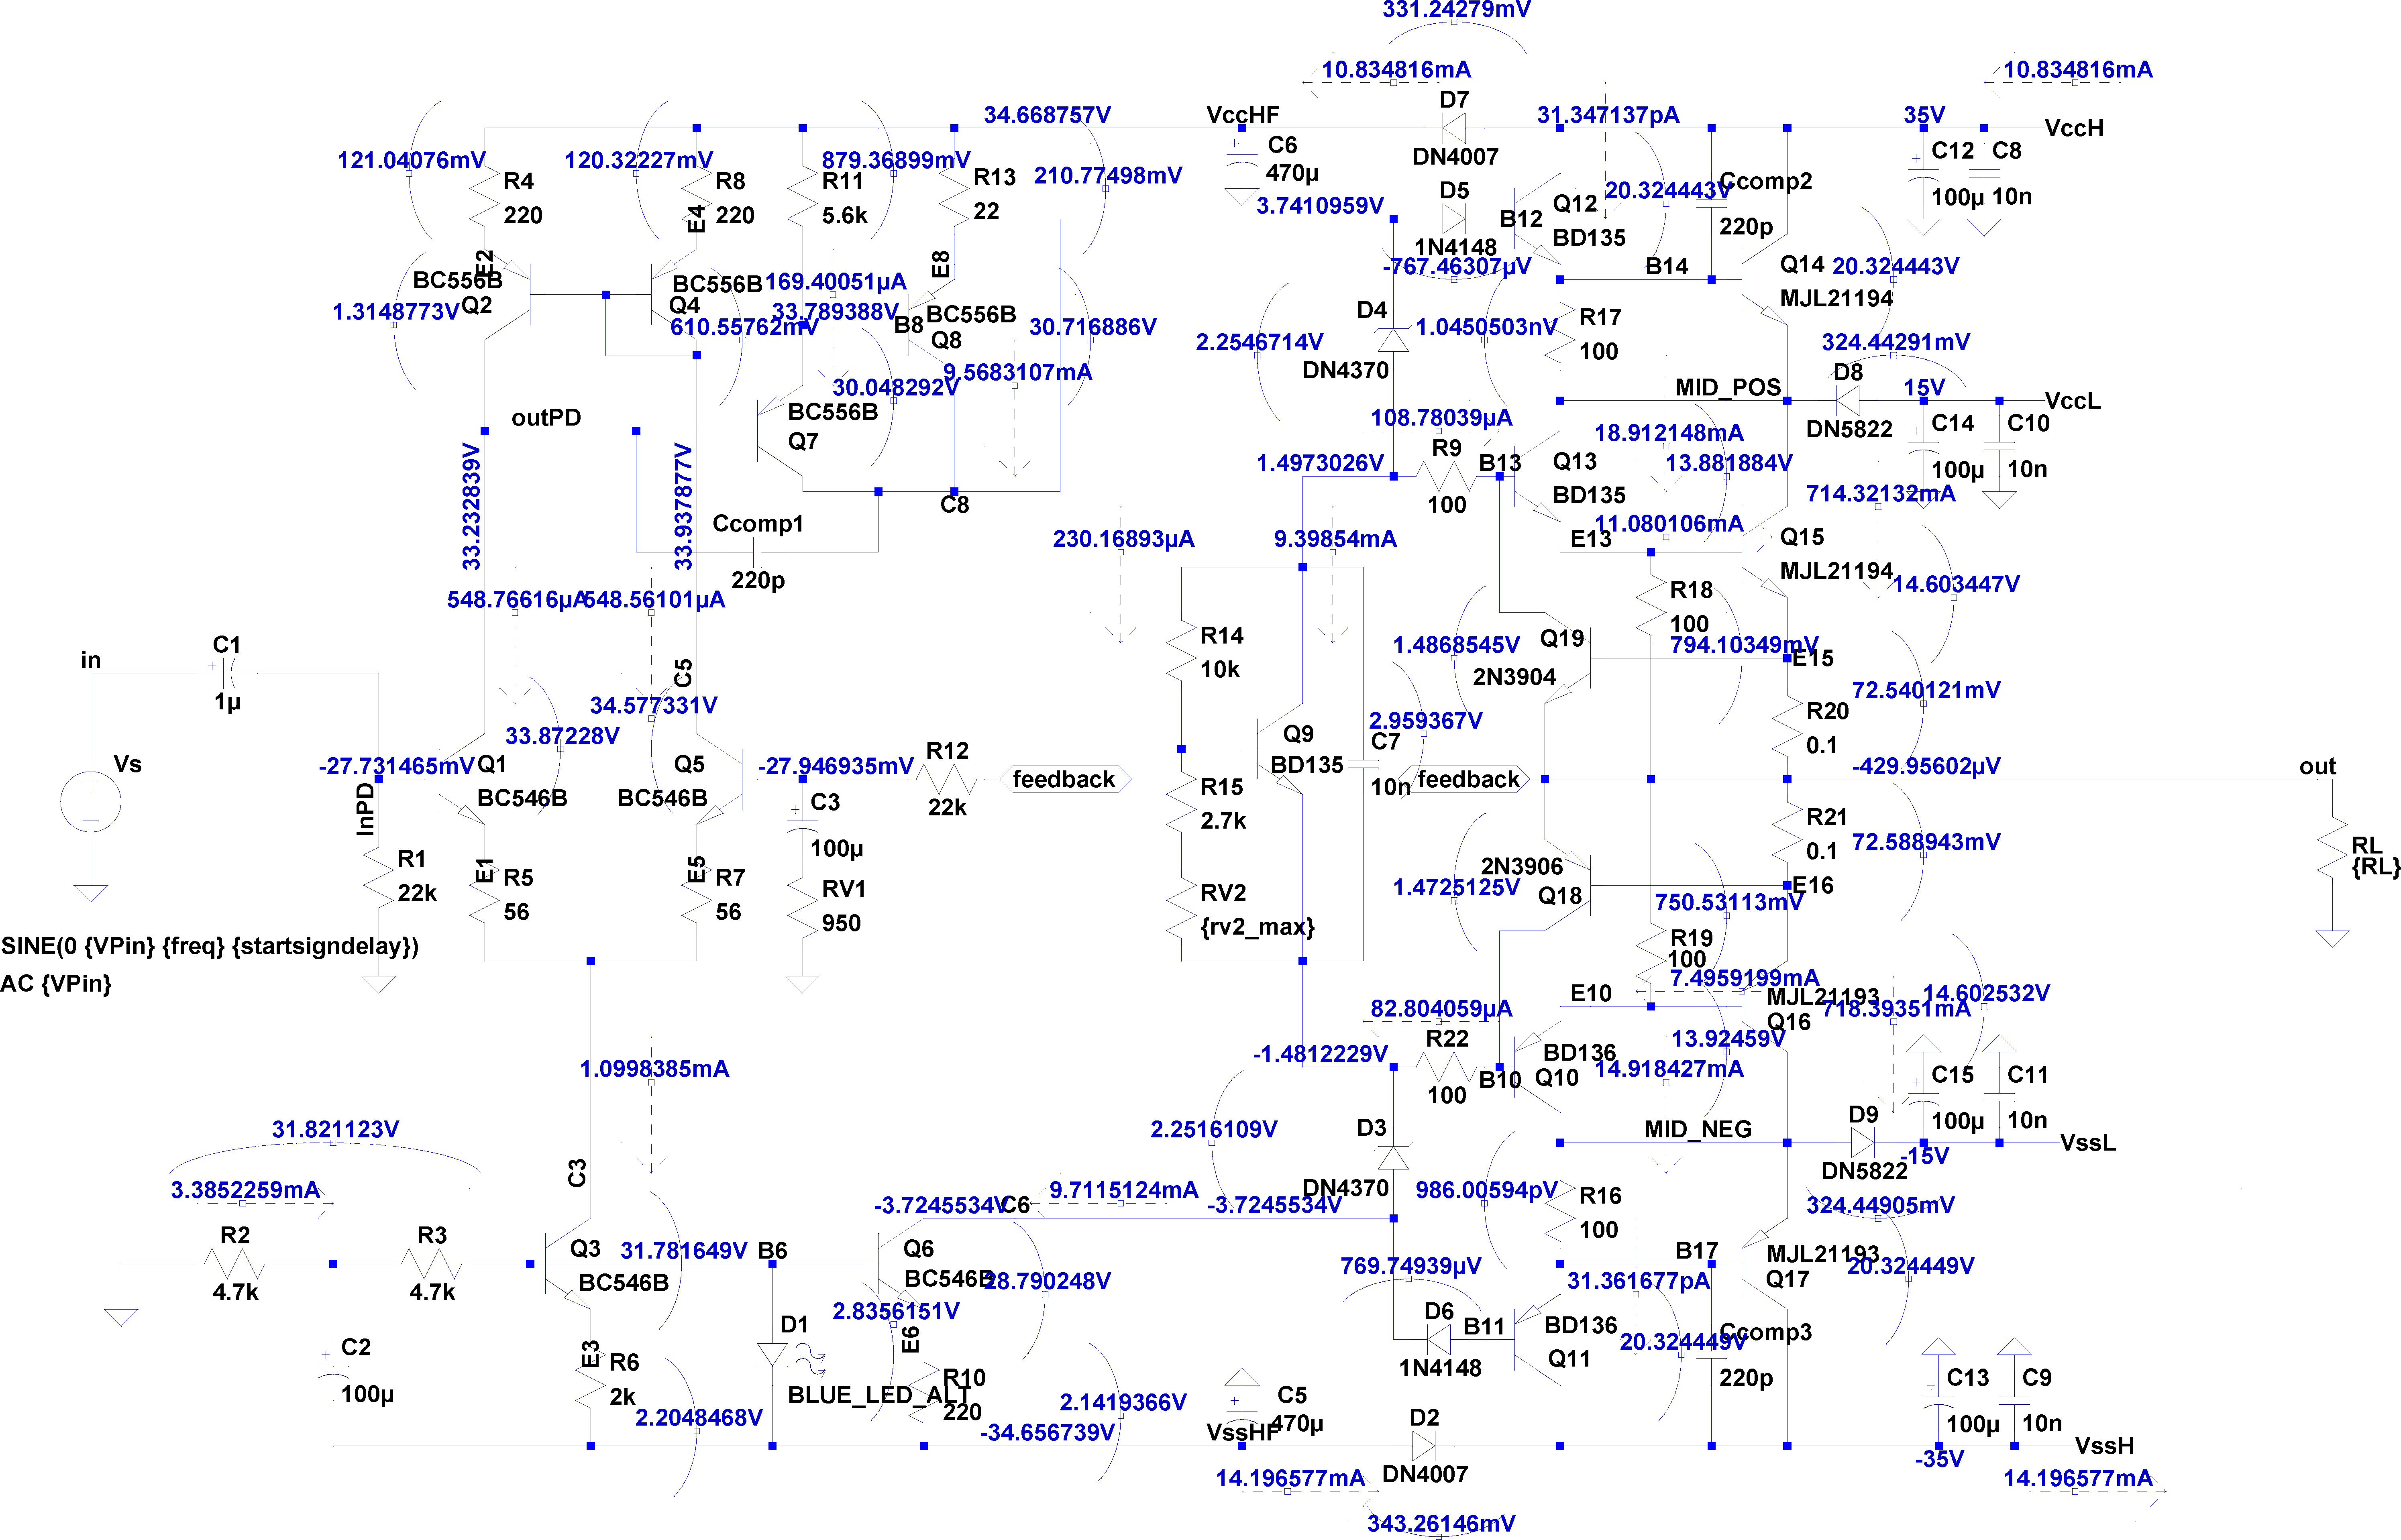
\includegraphics[height=0.77 \textwidth, angle=90]{./img/circuito/amplifier.png}
    \caption{Circuito simulado mostrando los valores de polarización.}
    \label{fig:PuntoQ_simulacion}
\end{figure}

\clearpage

\subsection{Ganancia de lazo}

\par En la figura ~\figref{fig:gain_loop_sim} se puede observar la ganancia de lazo del circuito, simulado a distintas frecuencias. A su vez, se especifica el margen de ganancia y de fase, para verificar la correcta estabilización del circuito. Obteniéndose de este modo:

\begin{itemize}
    \item Margen de ganancia: $29.21 \si[per-mode=symbol]{\decibel}$
    \item Margen de fase: $86.12 \si[per-mode=symbol]{\degree}$
\end{itemize}

\vfill

\clearpage

\begin{figure}[H]
    \centering
    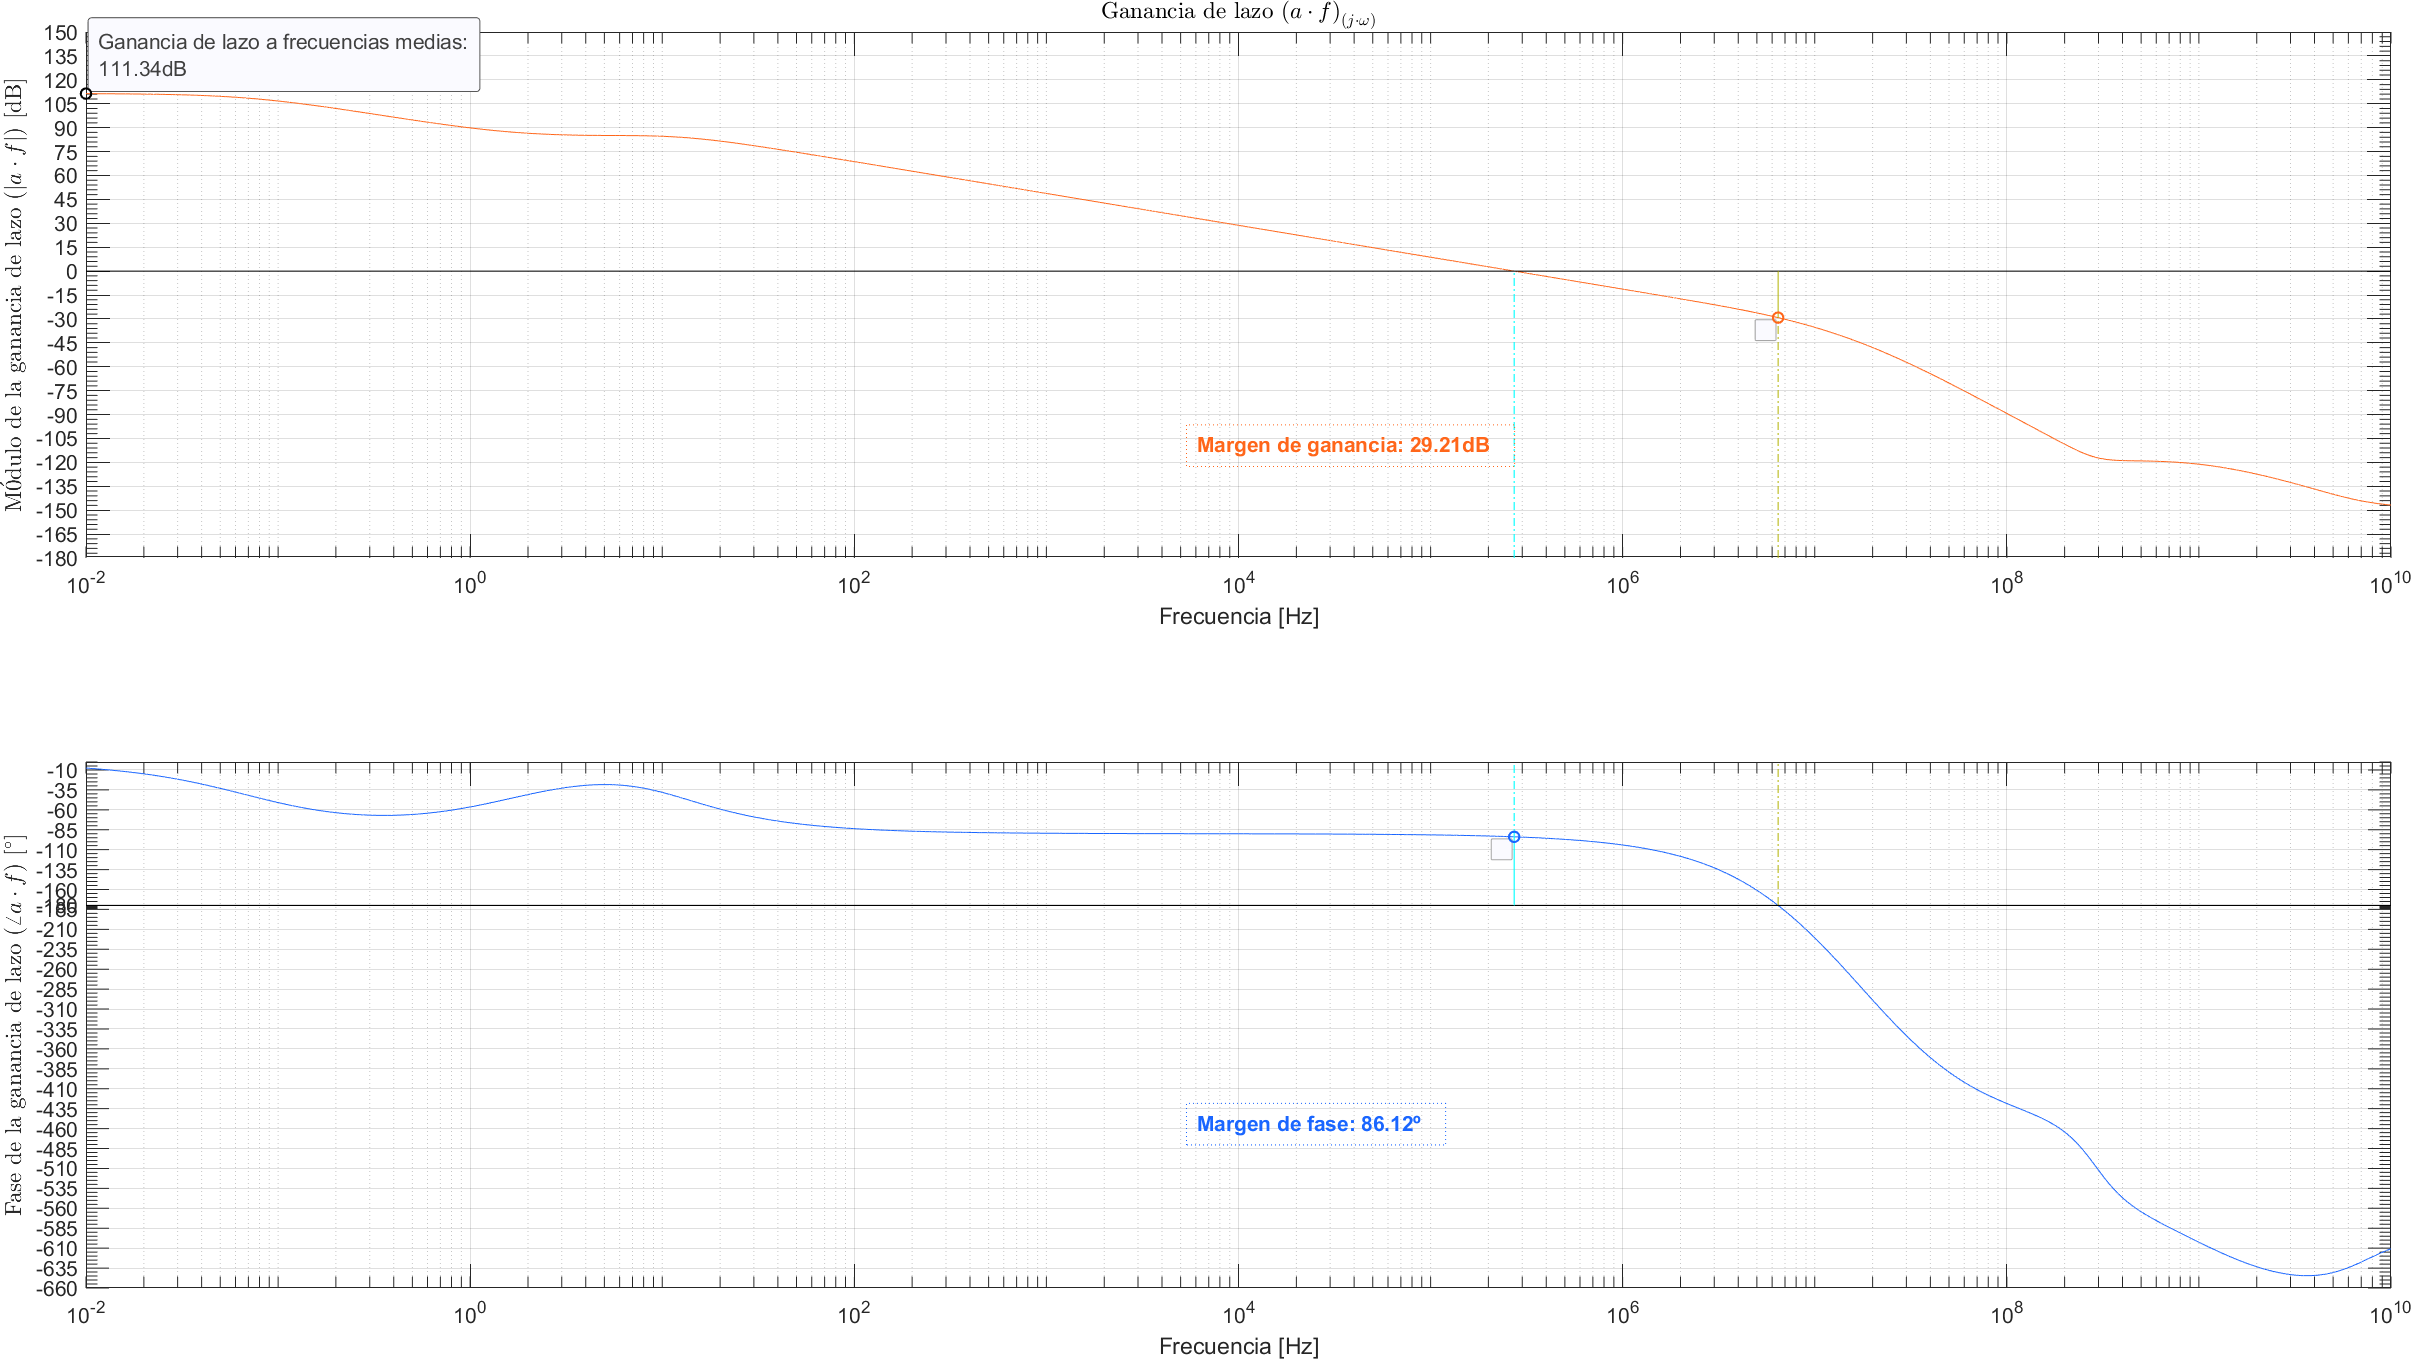
\includegraphics[height=0.66 \textwidth, angle=90]{./img/simulaciones/Loop/gain_loop.png}
    \caption{Ganancia de lazo (simulación).}
    \label{fig:gain_loop_sim}
\end{figure}

\clearpage

\subsection{Ancho de banda}

\par En la figura ~\figref{fig:Low_power_BW} se muestra el resultado de la simulación del ancho de banda del circuito.
\par Obtenemos un ancho de banda de $97.89kHz$ con frecuencias de corte:

\begin{itemize}
    \item $f_l =22.34 \si[per-mode=symbol]{\hertz}$
    \item $f_h =97.92 \si[per-mode=symbol]{\kilo\hertz}$
\end{itemize}

\vfill

\clearpage

\begin{figure}[H]
    \centering
    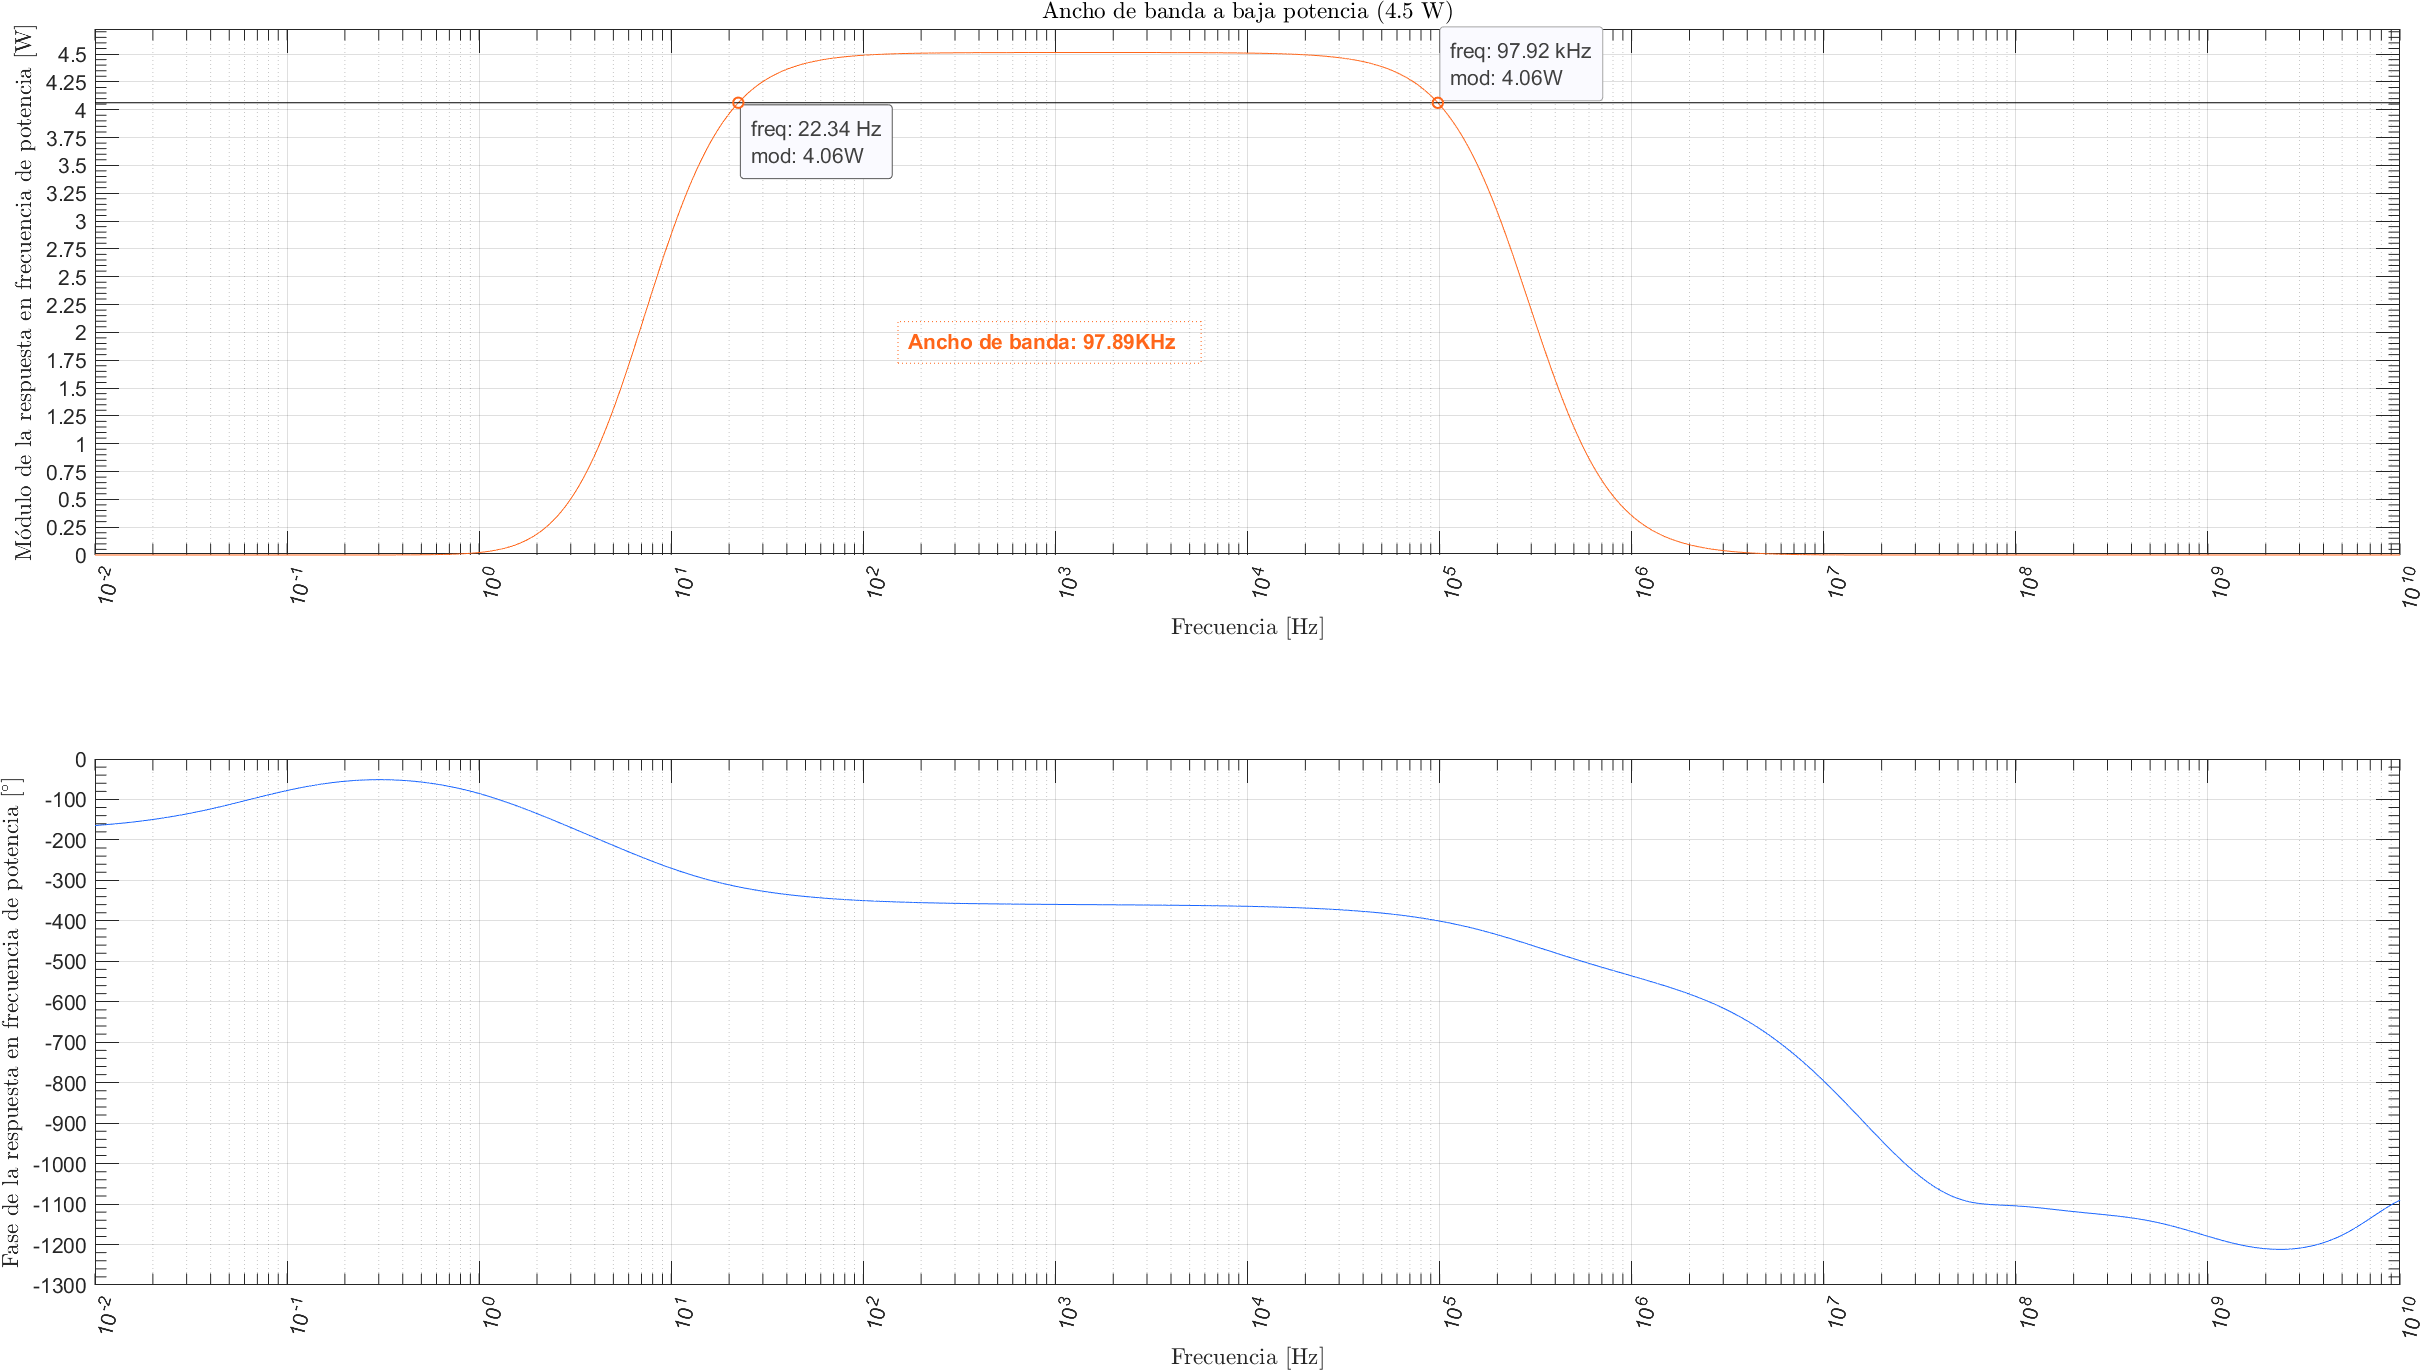
\includegraphics[height=0.66 \textwidth, angle=90]{./img/simulaciones/BW/Low_power_BW.png}    \caption{Ancho de banda a baja potencia (simulación).}
    \label{fig:Low_power_BW}
\end{figure}


\subsection{Ancho de banda de potencia}

\par En la figura ~\figref{fig:Power_BW_sim}, se observa el resultado de la simulación del ancho de banda de potencia simulado.
\par Obtenemos en el circuito un ancho de banda de potencia de $97.89kHz$ con frecuencias de corte:

\begin{itemize}
    \item $f_l = 22.34 \si[per-mode=symbol]{\hertz}$
    \item $f_h = 97.84 \si[per-mode=symbol]{\kilo\hertz}$
\end{itemize}

\vfill

\clearpage

\begin{figure}[H]
    \centering
    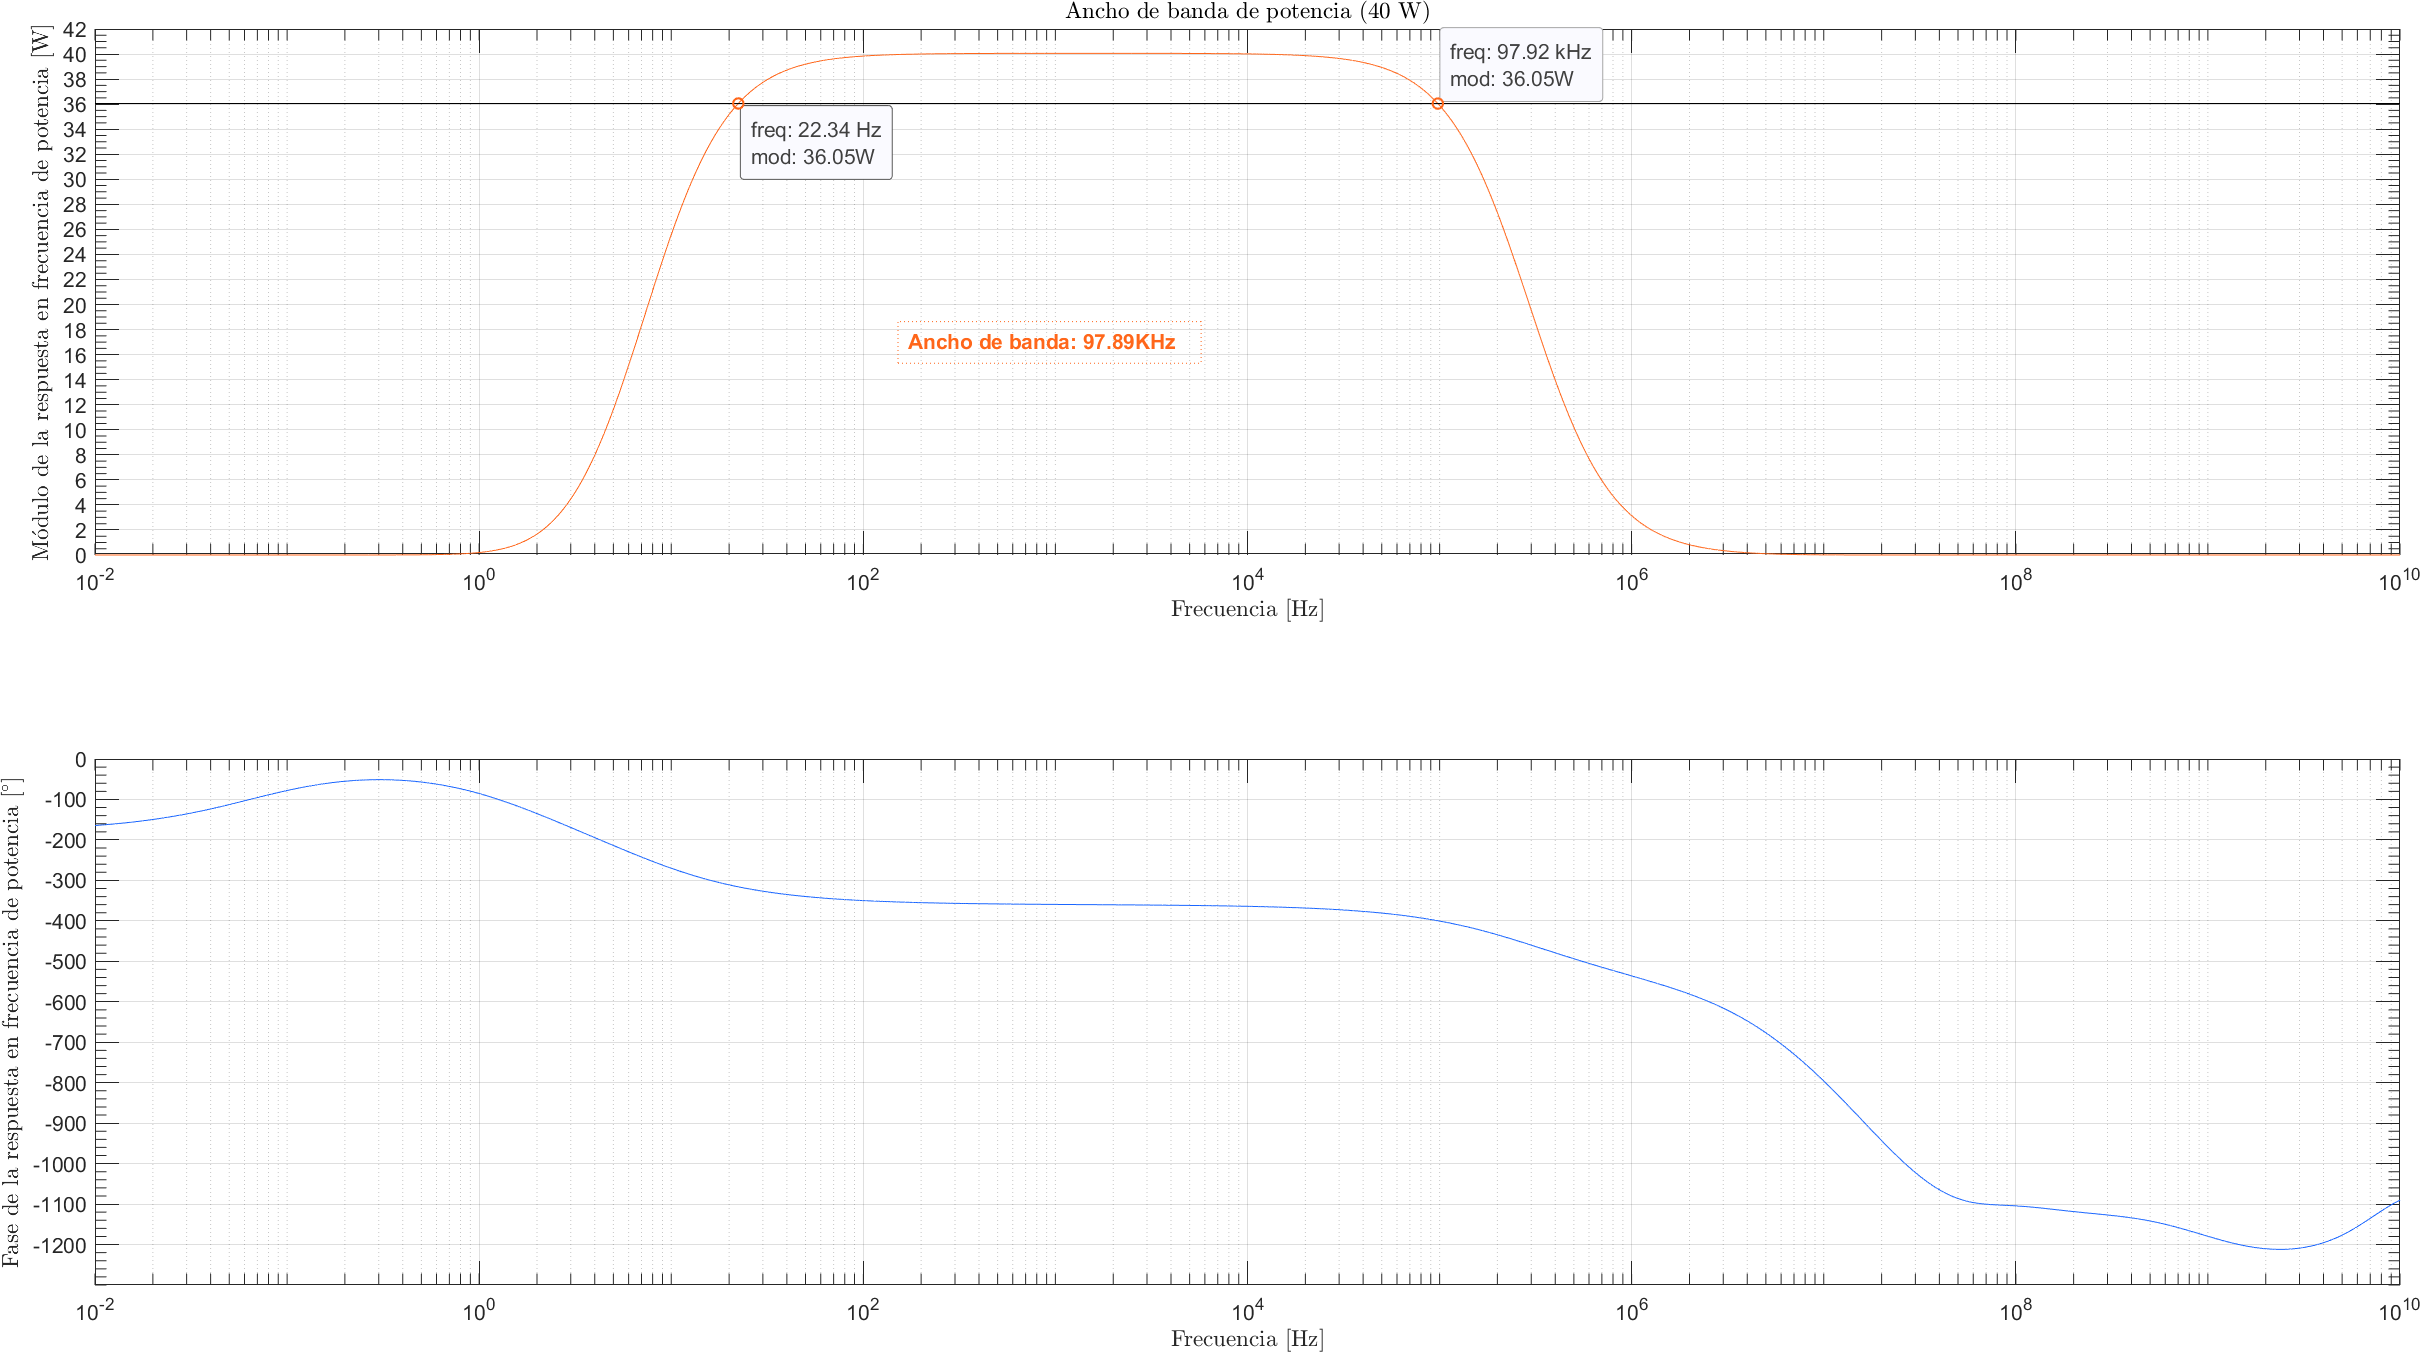
\includegraphics[height=0.66 \textwidth, angle=90]{./img/simulaciones/BW/Power_BW.png}
    \caption{Ancho de banda de potencia (simulación).}
    \label{fig:Power_BW_sim}
\end{figure}

\clearpage

\subsection{Impedancias de entrada y salida}

\par En las figuras ~\figref{fig:amplifier_Zi_sim} y ~\figref{fig:amplifier_Zo_sim} , se observa los valores de la resistencia de entrada y salida del amplificador, respectivamente, en función de la frecuencia.

\vfill

\clearpage

\begin{figure}[H]
    \centering
    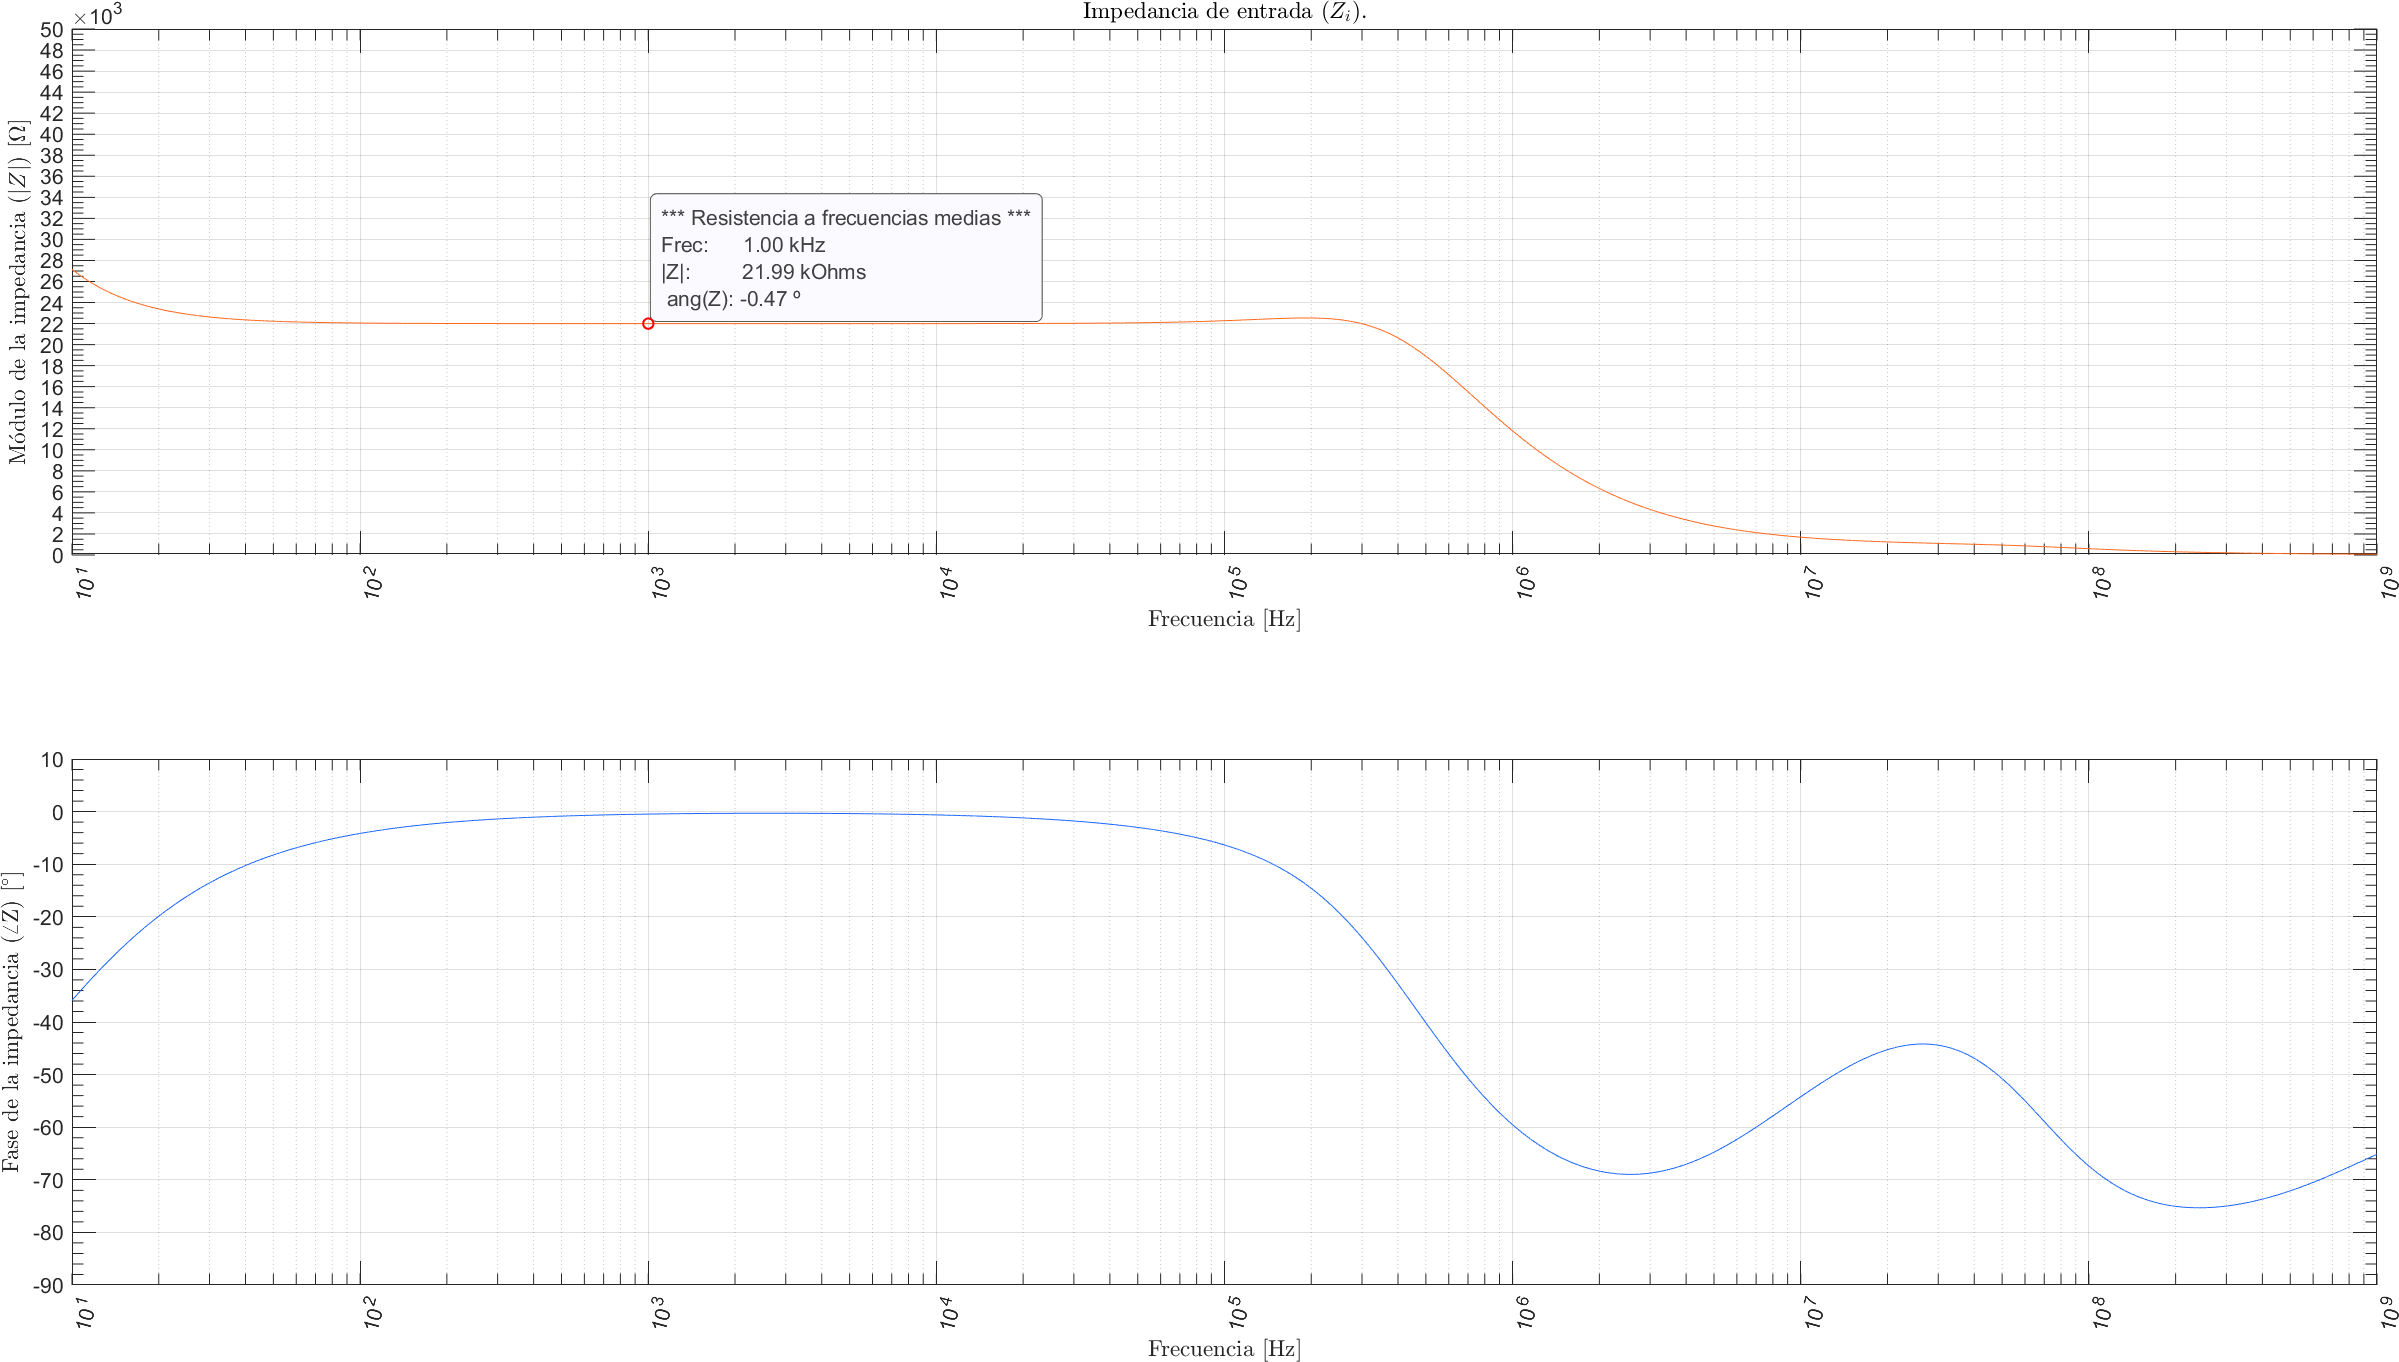
\includegraphics[height=0.66 \textwidth, angle=90]{./img/simulaciones/Impedance/amplifier_Zi.png}
    \caption{Valores de impedancia de entrada (simulación).}
    \label{fig:amplifier_Zi_sim}
\end{figure}

\clearpage

\begin{figure}[H]
    \centering
    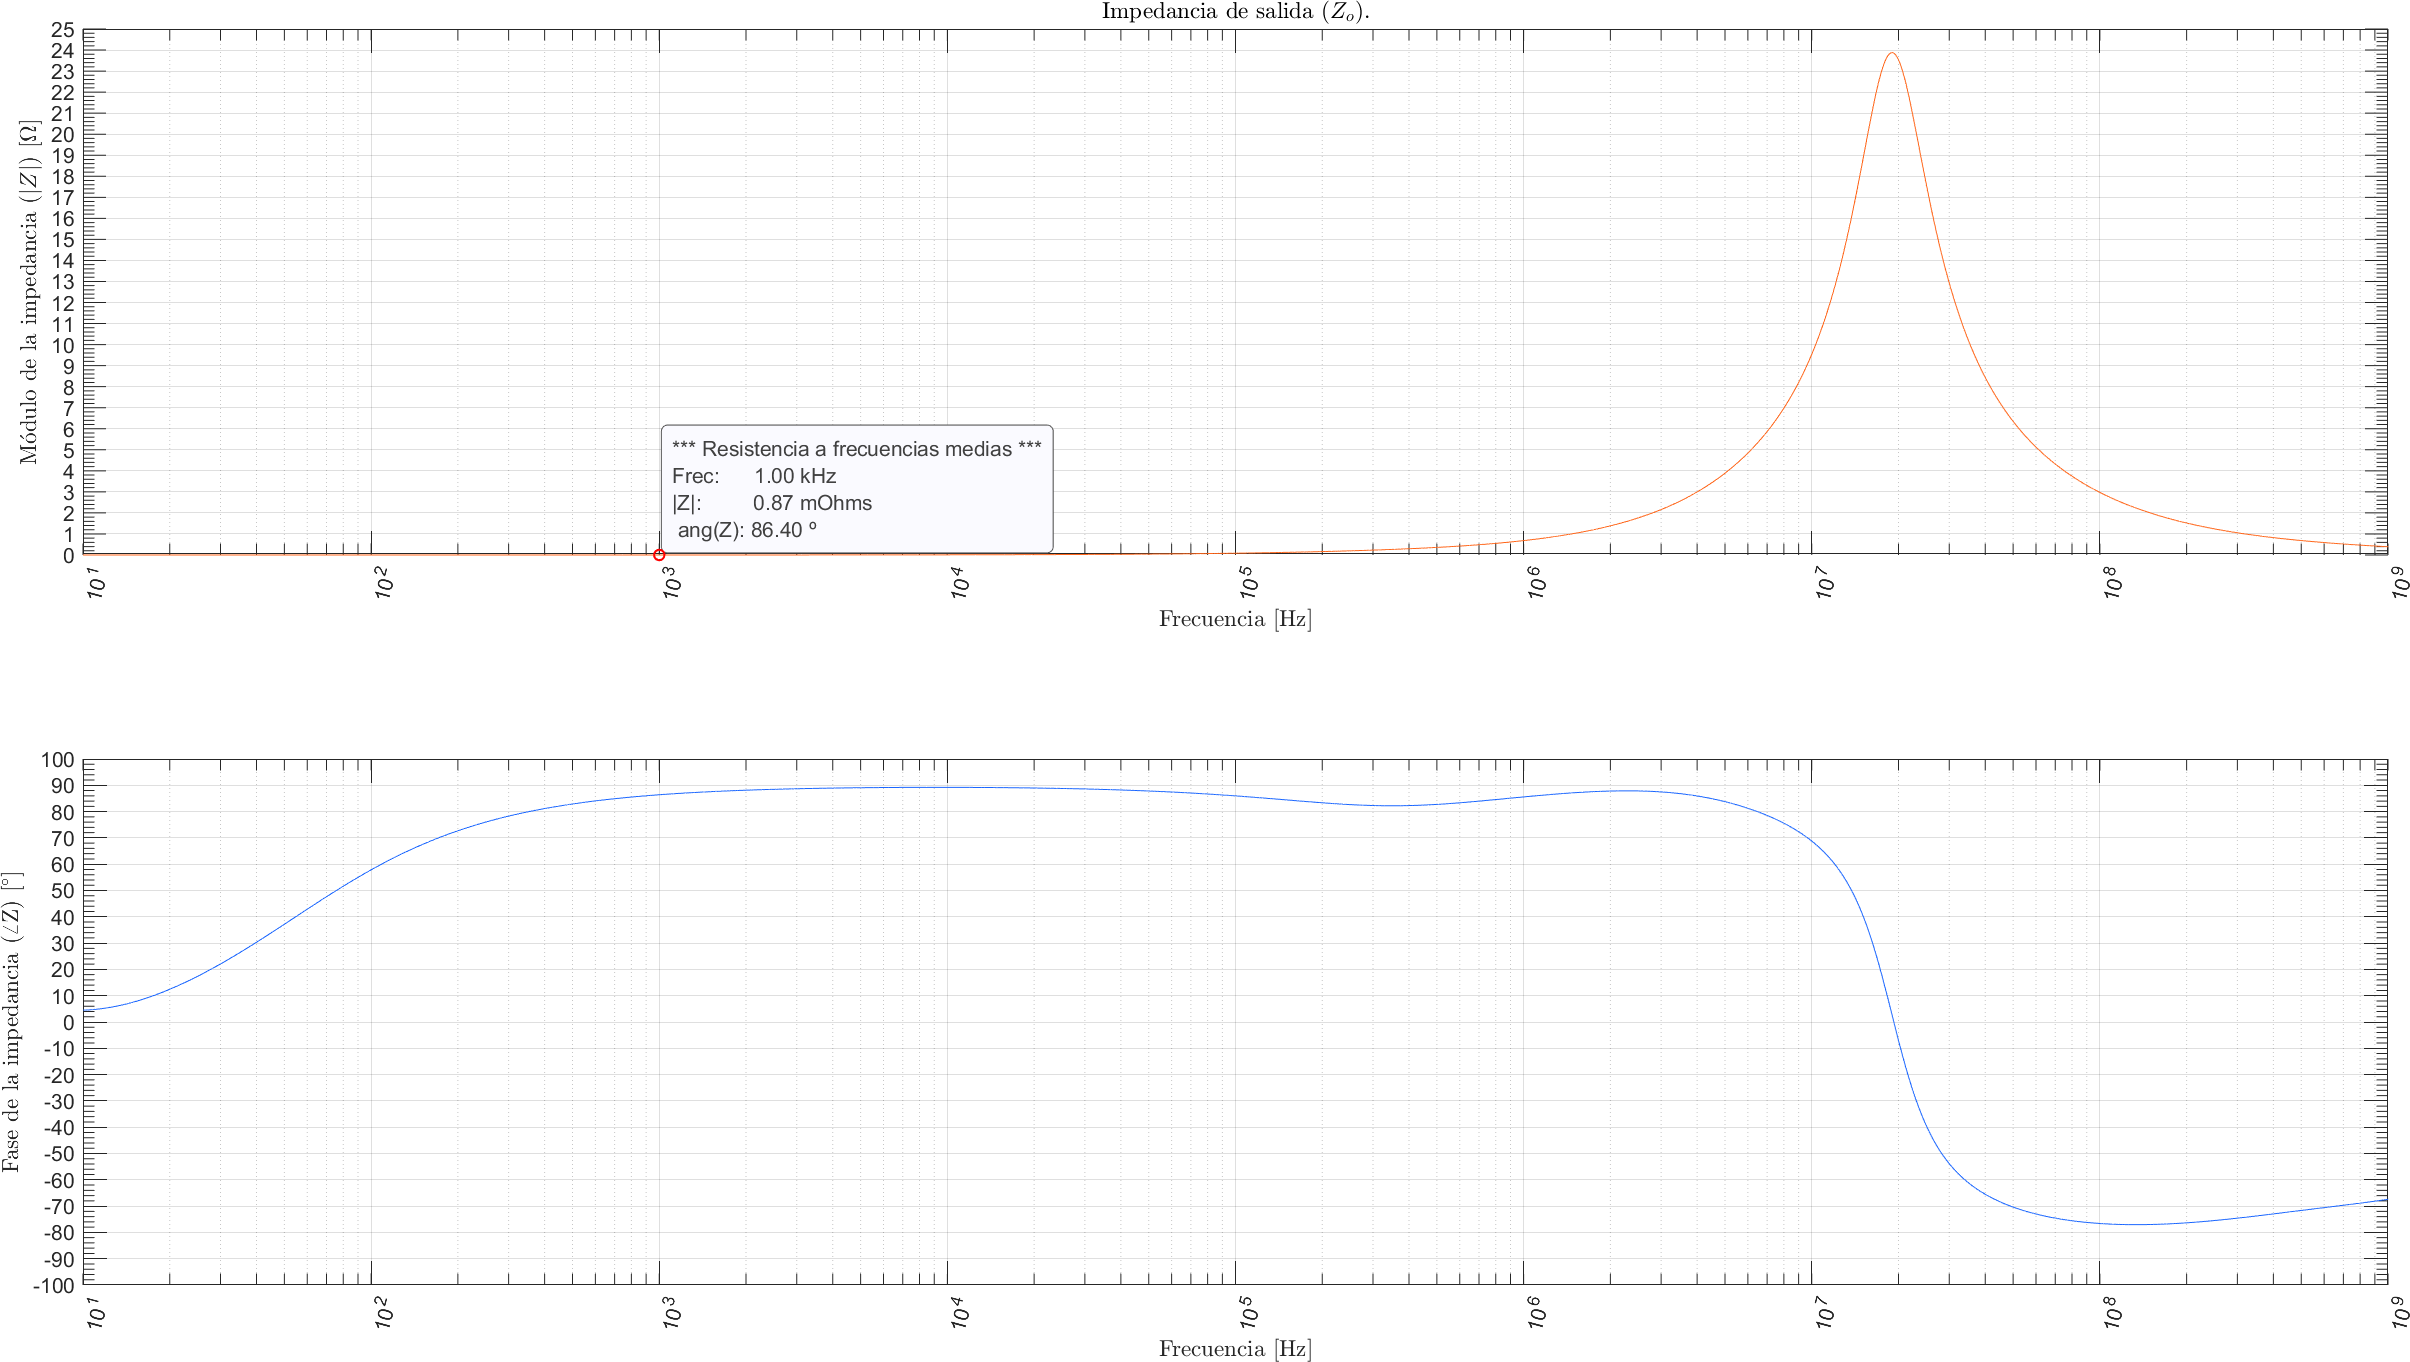
\includegraphics[height=0.66 \textwidth, angle=90]{./img/simulaciones/Impedance/amplifier_Zo.png}
    \caption{Valores de impedancia de salida (simulación).}
    \label{fig:amplifier_Zo_sim}
\end{figure}

\clearpage

\subsection{THD}

\begin{figure}[H]
    \centering
    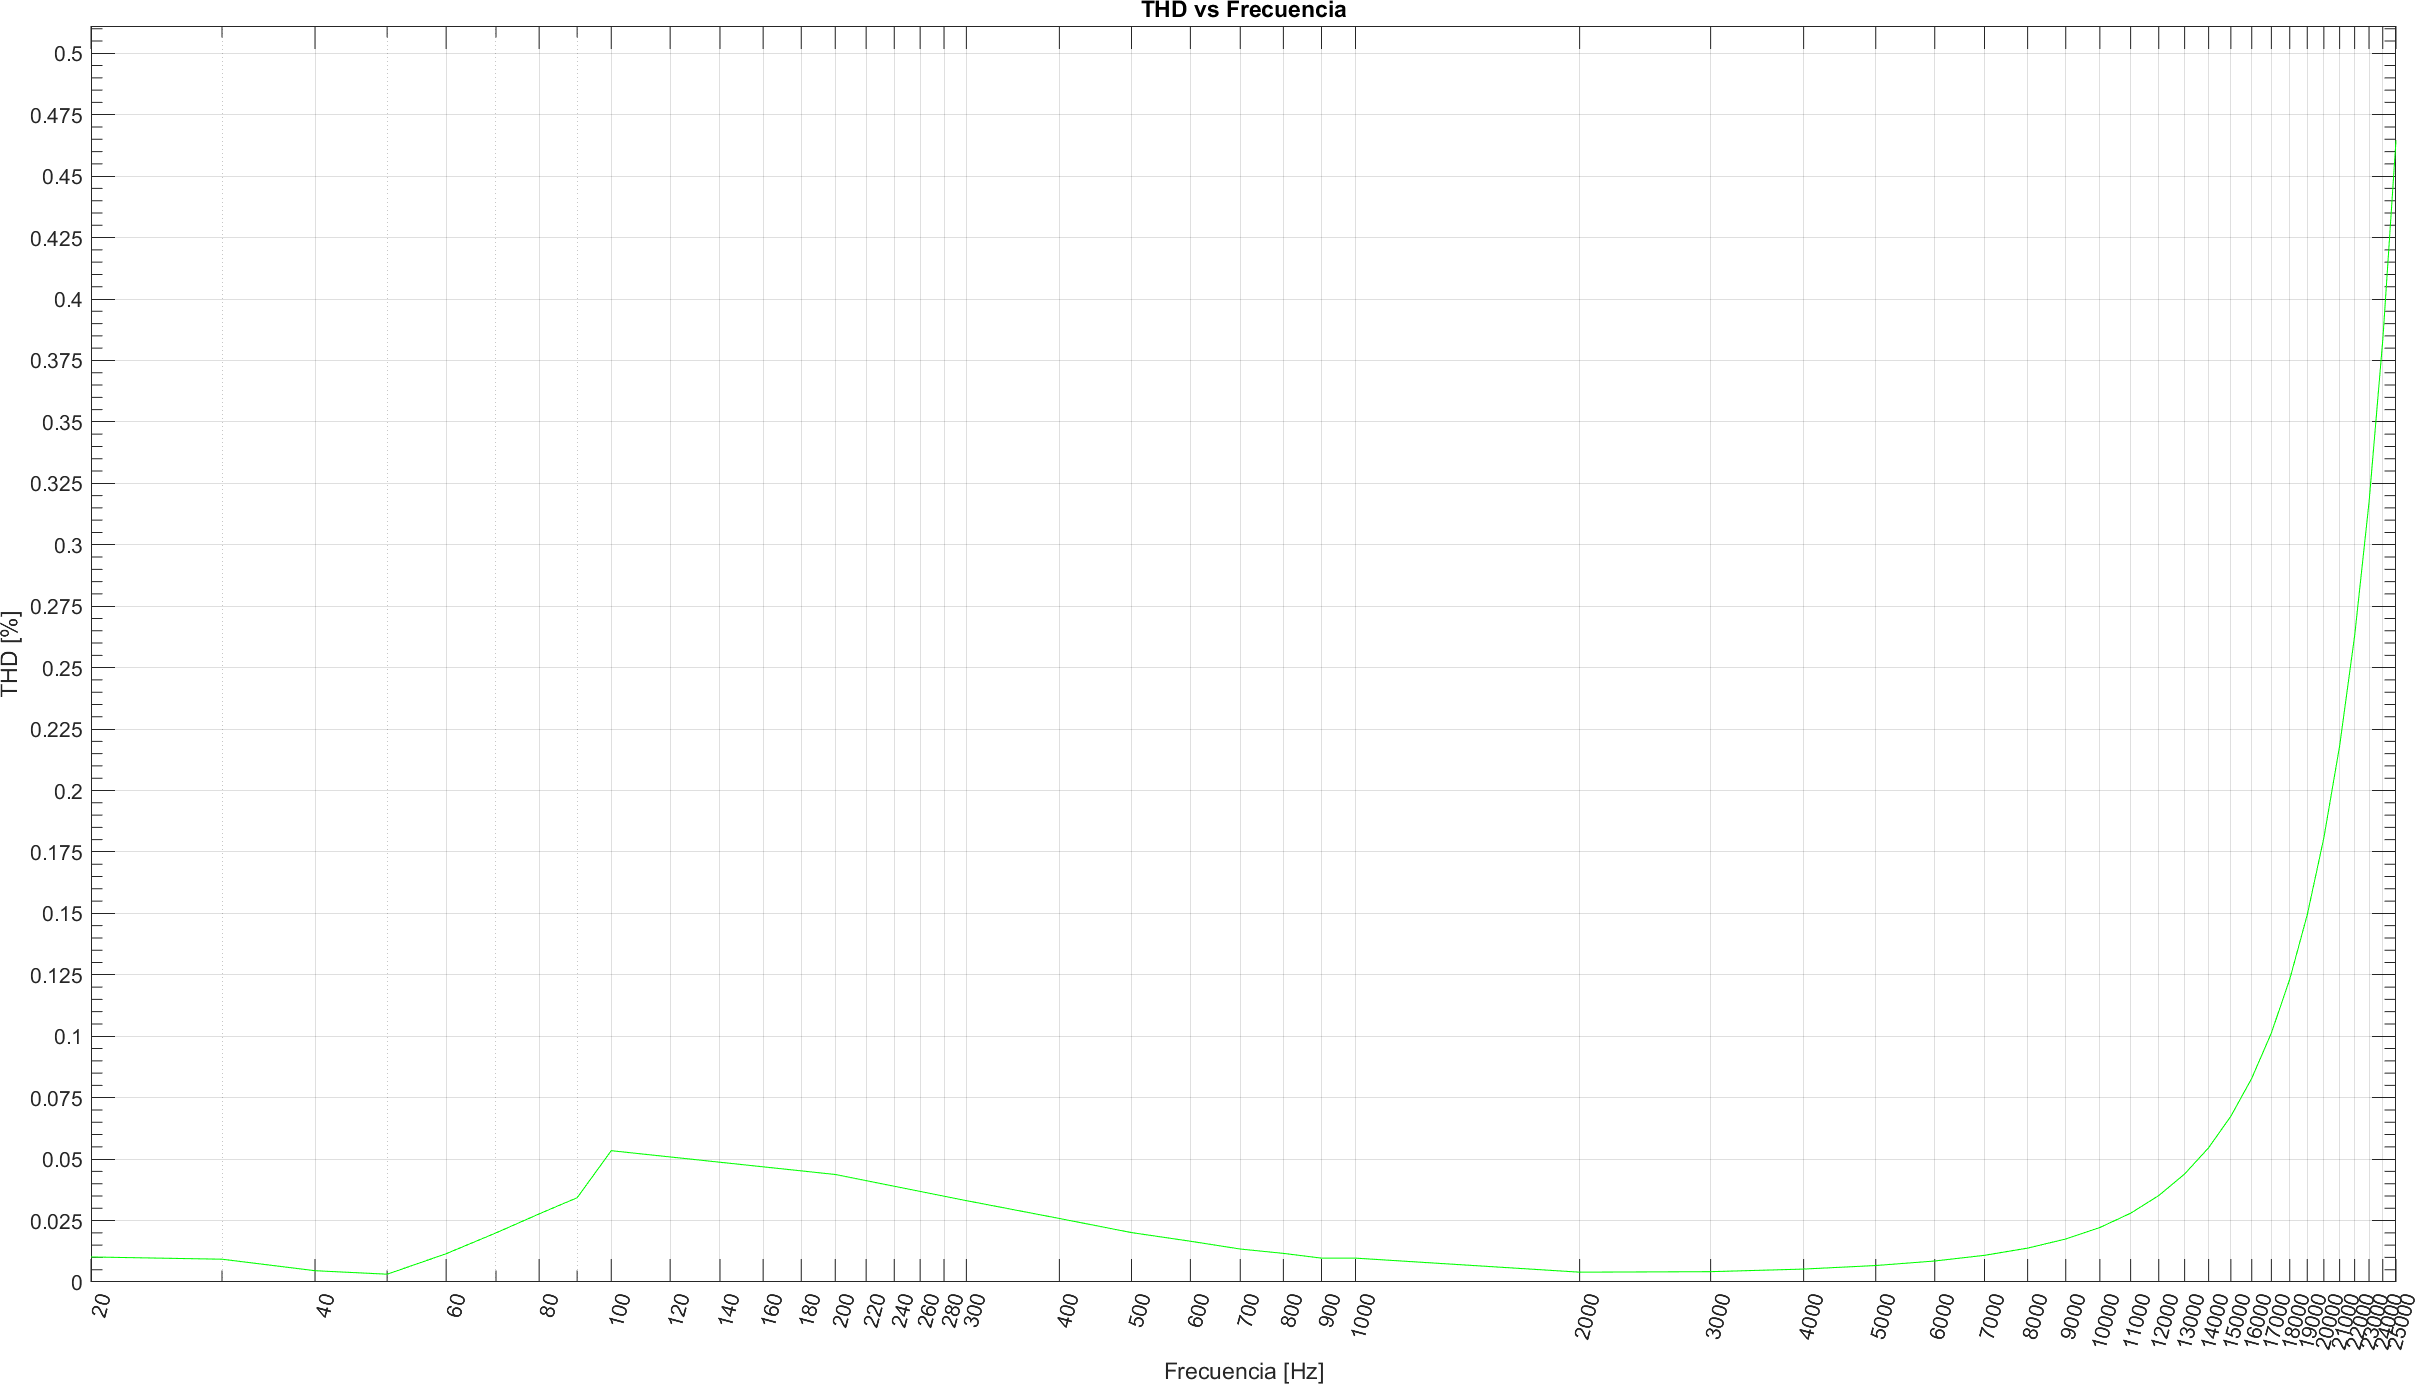
\includegraphics[height=0.66 \textwidth, angle=90]{./img/simulaciones/THD/THD_vs_frequency_sim.png}
    \caption{THD en función de la frecuencia (simulación).}
    \label{fig:THD_vs_frequency_sim}
\end{figure}

\clearpage

\begin{figure}[H]
    \centering
    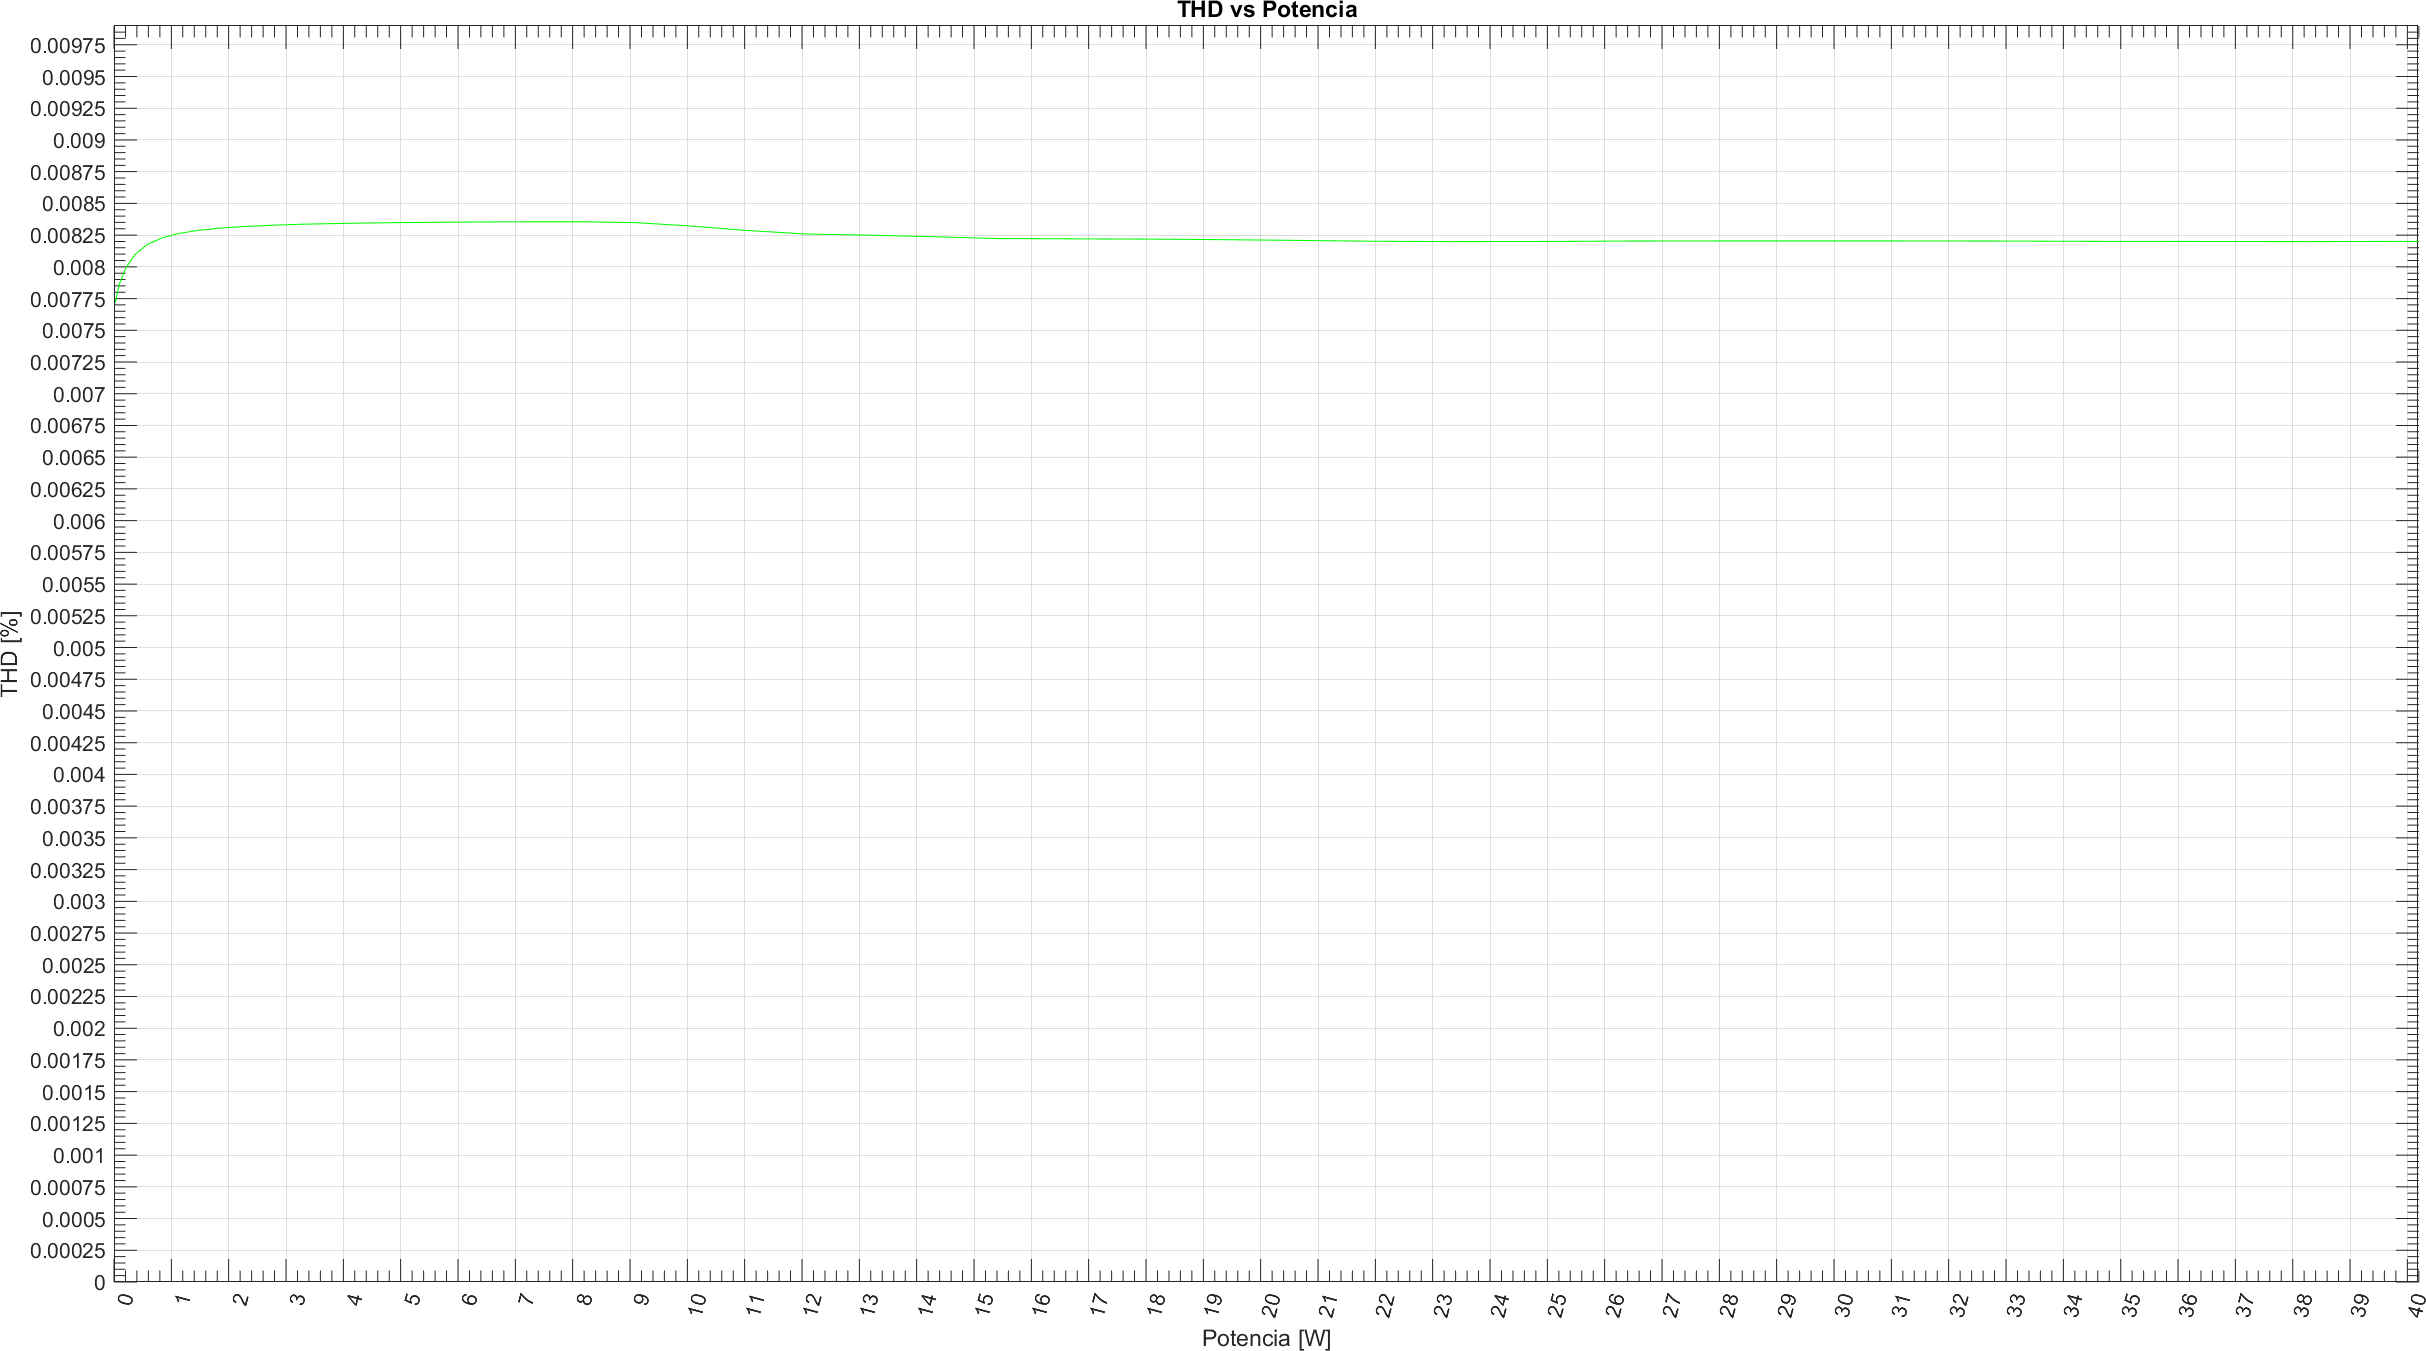
\includegraphics[height=0.66 \textwidth, angle=90]{./img/simulaciones/THD/THD_vs_power_sim.png}
    \caption{THD en función de la potencia (simulación).}
    \label{fig:THD_vs_power_sim}
\end{figure}

\clearpage

\subsection{Slew Rate}

\par En la figura ~\figref{fig:Slew_Rate} observamos el resultado de la simulación utilizada para el cálculo del Slew Rate. En la figura  ~\figref{fig:Slew_Rate_zoom}, se aprecia con más claridad la pendiente para el cálculo, además del efecto que produce la conmutación entre las fuentes de $15 \si[per-mode=symbol]{\volt}$ y $35 \si[per-mode=symbol]{\volt}$.

\par A partir del cálculo de la pendiente producida por la respuesta al escalón obtenemos como resultado del Slew Rate:

\begin{itemize}
    \item Slew Rate = $4.79 \si[per-mode=symbol]{\volt\per\micro\second}$
\end{itemize}

\vfill

\clearpage

\begin{figure}[H]
    \centering
    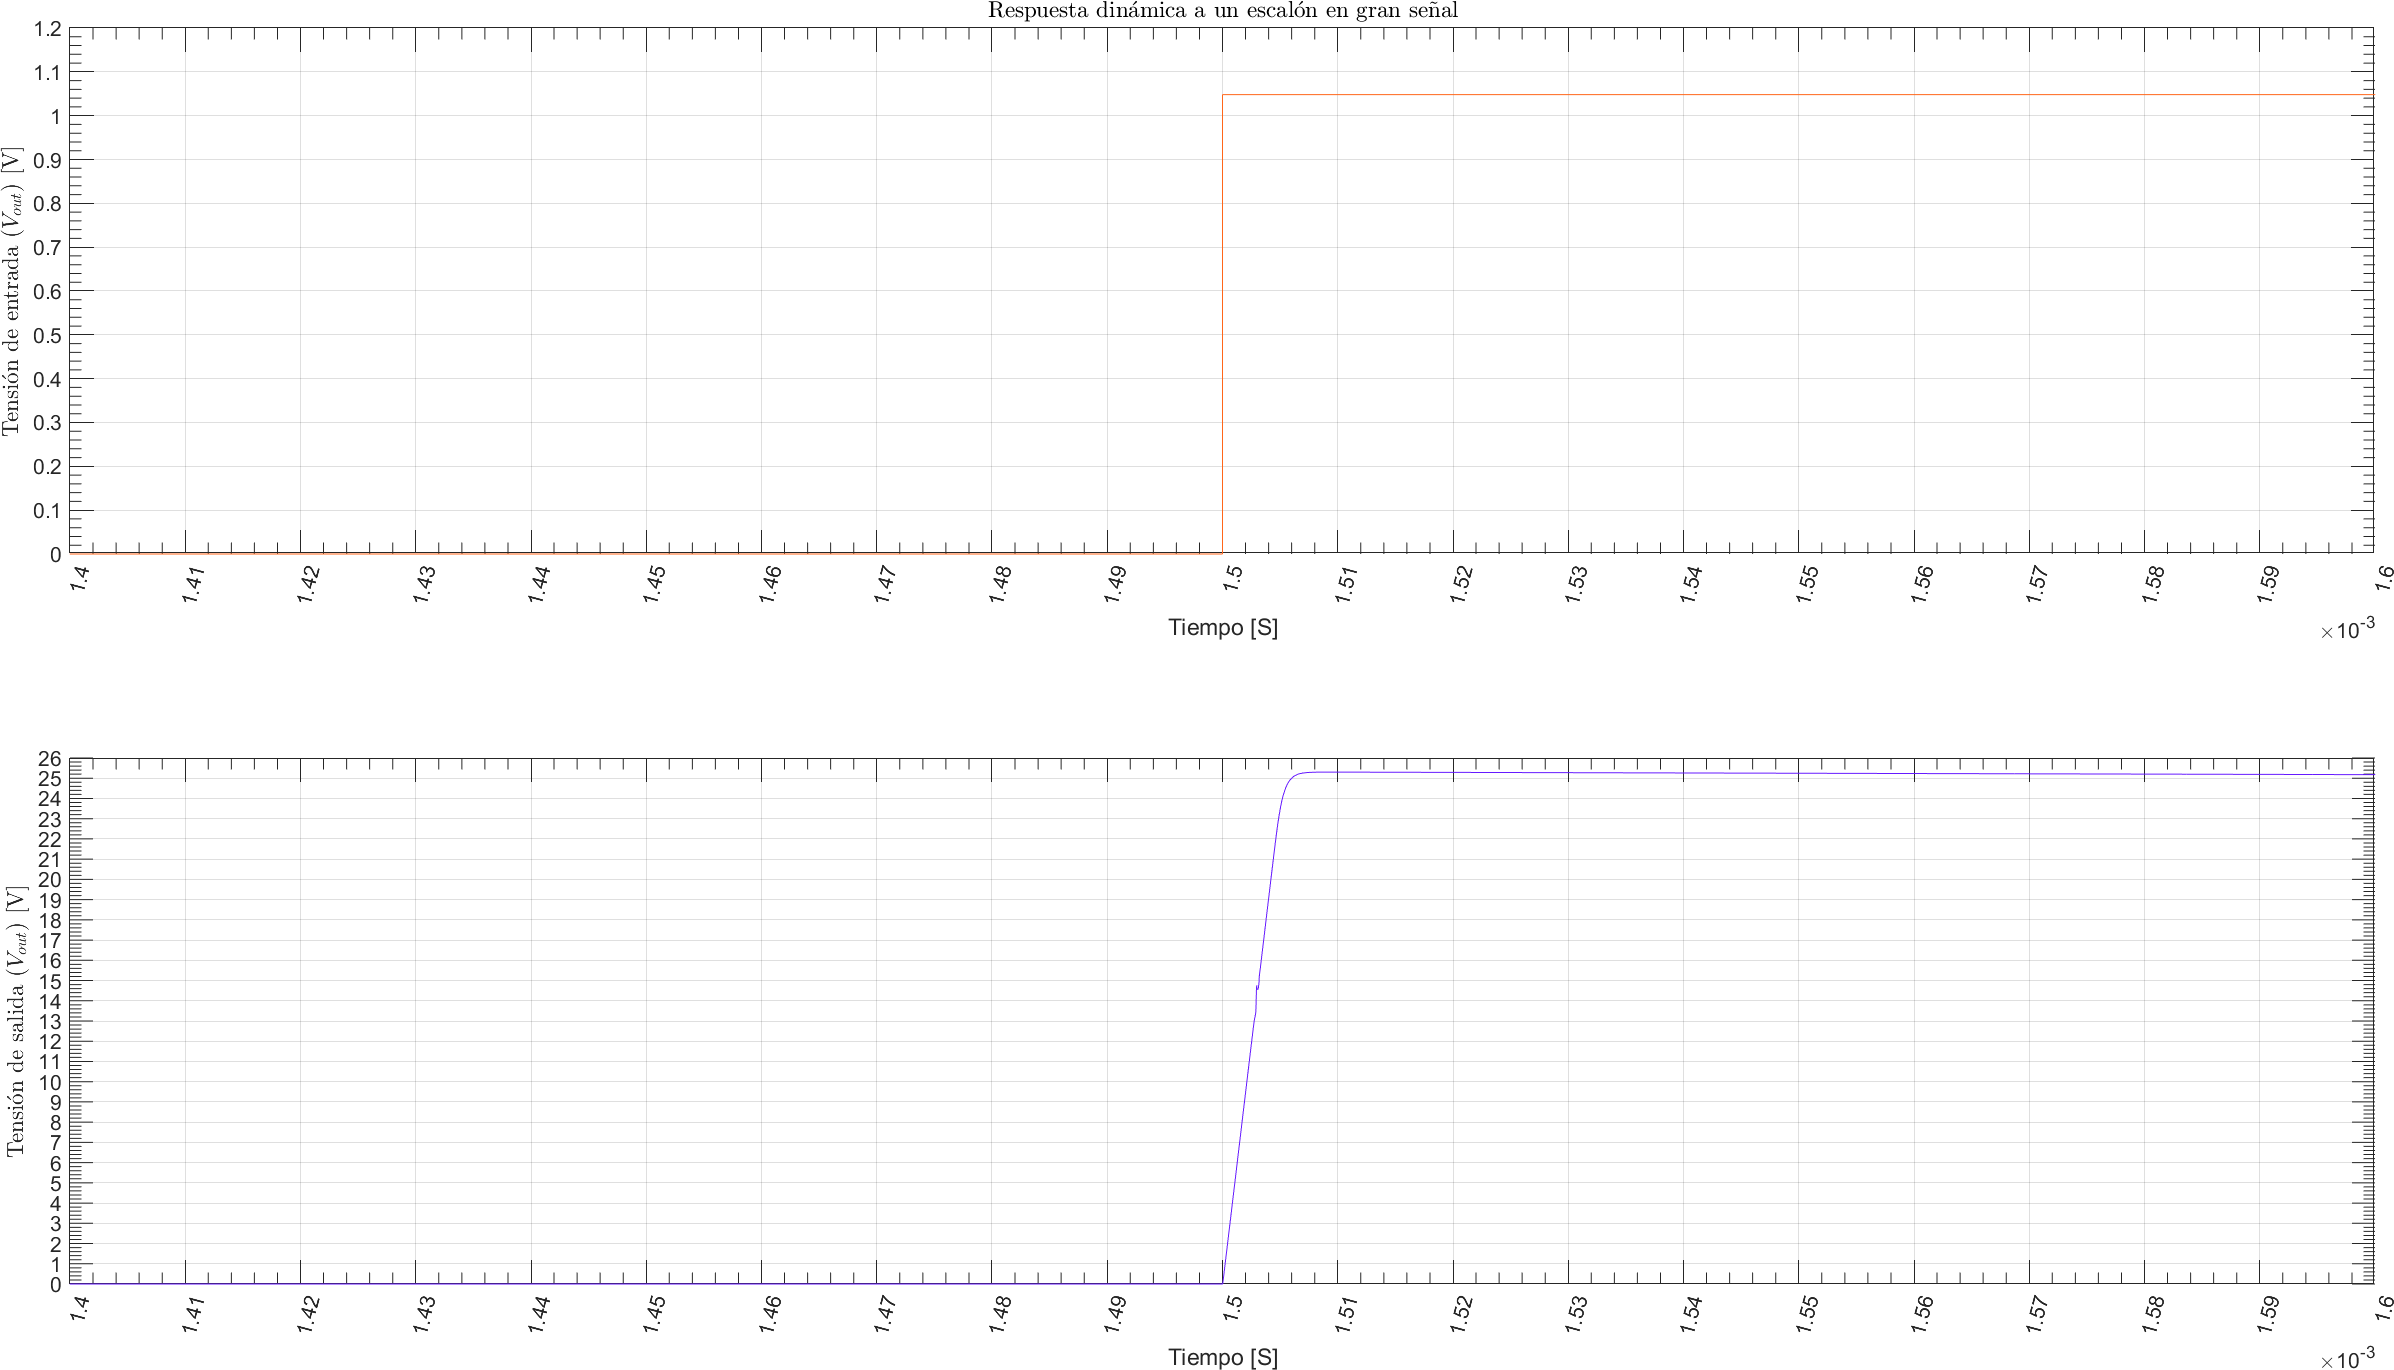
\includegraphics[height=0.66 \textwidth, angle=90]{./img/simulaciones/Slew_Rate/Slew_Rate.png}
    \caption{Tiempo de crecimiento (simulación).}
    \label{fig:Slew_Rate}
\end{figure}

\clearpage

\begin{figure}[H]
    \centering
    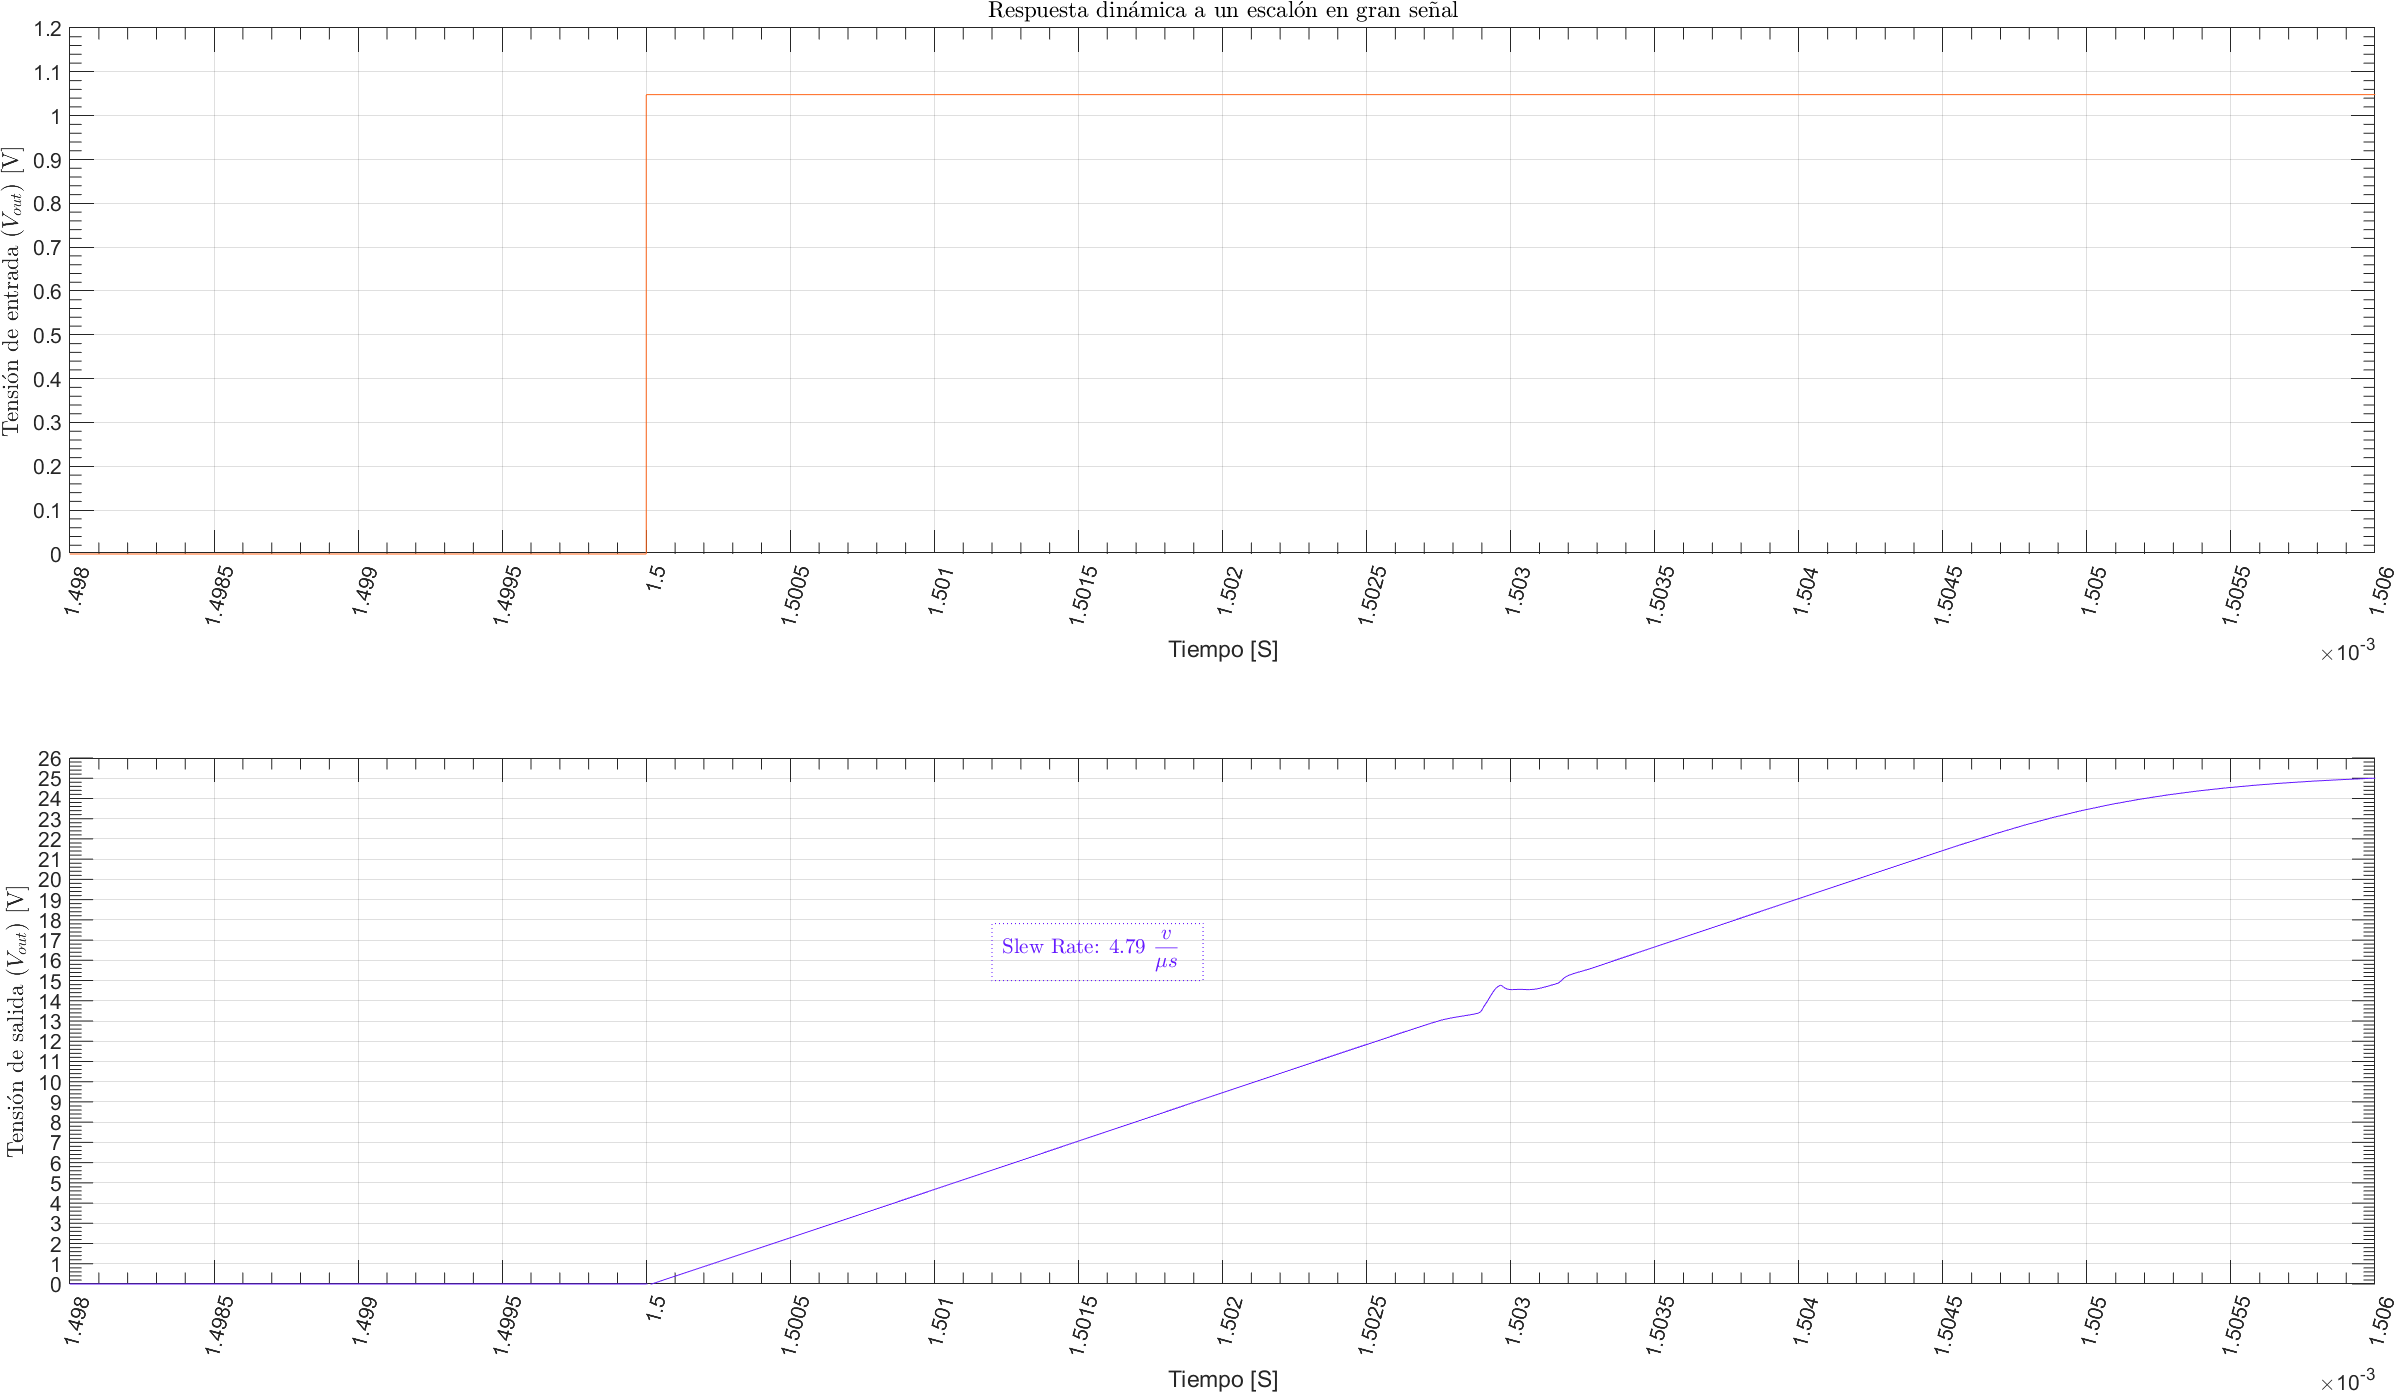
\includegraphics[height=0.66 \textwidth, angle=90]{./img/simulaciones/Slew_Rate/amplifier_SR_zoom.png}
    \caption{Tiempo de crecimiento, zoom sobre la pendiente  (simulación).}
    \label{fig:Slew_Rate_zoom}
\end{figure}

\clearpage